\chapter{内存管理}\label{OS03}

\par\medskip\noindent\textbf{章节脉络}\par\smallskip
\begin{wideblock}\centering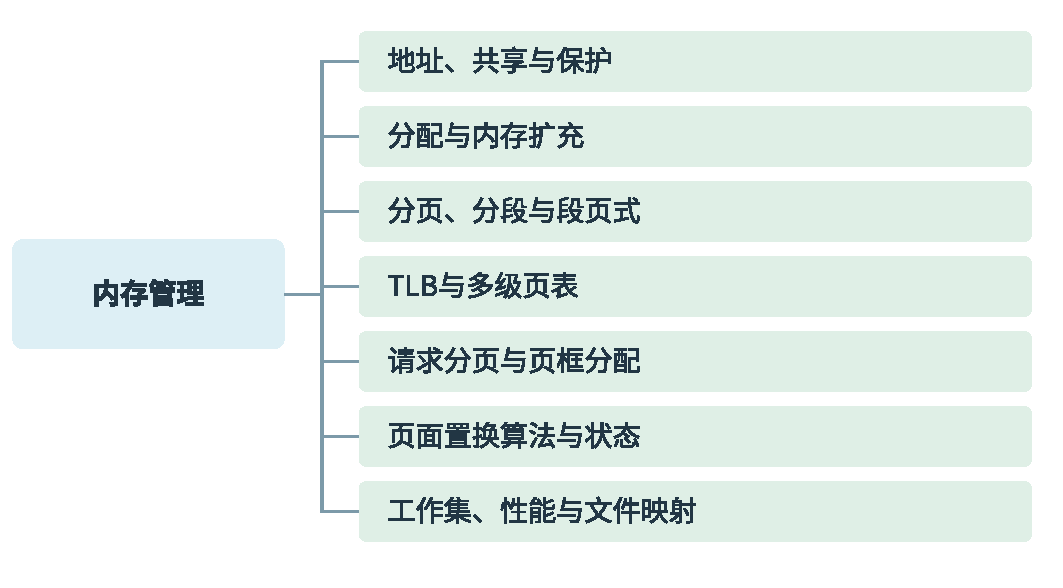
\includegraphics[width=\linewidth,height=92mm,keepaspectratio]{figures/overview.pdf}\end{wideblock}\par\medskip

\section{地址、驻留、权限与访问代价}\label{OS03-guide}

\begin{methodbox}[地址与缺页综合题的顺序]

\begin{enumerate}
\def\labelenumi{\arabic{enumi}.}
\tightlist
\item
  写明编址单位、地址位数、页大小和表项长度，先按二进制位宽拆分字段。
\item
  检查范围与权限，再根据TLB、各级页表的状态寻找有效映射。
\item
  遇合法但不驻留的页面，跟踪空闲页框、置换、脏页回写、映射更新和原指令重试。
\item
  沿完整引用串保存状态；最后分别汇总缺页、置换、访存和设备I/O次数，并统一时间单位。
\end{enumerate}

\end{methodbox}

\begin{definition}[一次访存要回答三个独立问题]

地址是否属于合法范围、页面此刻是否驻留、当前操作是否有权限，是三个独立判断。页号用于查映射，页内偏移定位页中的字节；页表项的位置也不是最终数据的位置。

\end{definition}

\Needspace{120pt}

\subsection{页内偏移为何保持不变}\label{OS03-offset-proof}

\begin{proof}[从整数除法得到地址分解]

页大小为\(P\)字节时，任意非负字节地址\(a\)唯一写成\(a=pP+w\)，其中\(0\le w<P\)。页表把第\(p\)页整体映射到第\(f\)页框，页内第\(w\)个字节便落在\(fP+w\)。因此转换只替换页的整体位置，不改变页内坐标；只有\(P=2^d\)时，才可直接把偏移解释为低\(d\)个二进制位。

\end{proof}

\section{内存扩充：覆盖、交换与请求调页}\label{OS03-extension}

覆盖、交换和按需分页都在缓解内存容量限制，但管理对象与实施条件不同。\textbf{覆盖}把不会同时使用的程序段安排到同一覆盖区，在需要时替换，通常要求事先分析模块调用关系；常驻部分与覆盖区应共同满足执行需求。它并非把任意两个正要同时使用的模块强行放在一起。

\textbf{交换}按经典模型把暂不执行的进程整体或较大运行映像换到后备存储，需要时再换入；换出与进程阻塞不是同一概念，挂起状态用于表达不驻留。可否换出还受固定缓冲、正在进行的I/O与地址重定位等约束，不能随意移动设备仍在直接访问的内存。

\textbf{请求调页}把管理粒度缩小为页，合法页面可暂不驻留，真正引用时由缺页机制调入。它依赖页表状态、异常处理与后备关系，能够利用局部性；并不要求程序员预先列出覆盖模块。覆盖、交换和分页可以在不同层次讨论，不能仅凭``把内容移到磁盘''便认作同一种机制。

内存管理同时处理三个问题：程序用什么地址描述对象，这个地址此刻对应哪里，访问是否被允许。连续分配、分页和分段使用不同的映射单位；请求分页又允许某些合法内容暂不在物理内存。做题时先区分地址、映射和驻留状态，再进行位数或时间计算。

本章容量中的 KB、MB、GB 按题目所采用的二进制单位理解，即 \(2^{10}\)、\(2^{20}\)、\(2^{30}\) B；需要严格区分标准时可写 KiB、MiB、GiB。地址与页号、页框号从 0 编号；十六进制数以 H 结尾。页、页框大小相同；没有特别说明时，地址按字节编址。

\section{逻辑地址、物理地址和可寻址范围}\label{OS03-5-1}

\textbf{逻辑地址或虚拟地址}是程序在自身地址空间中使用的地址；\textbf{物理地址}标识主存中的实际位置。CPU 执行访存指令形成虚拟地址，地址变换机构按当前进程的映射得到物理地址，再访问主存。操作系统创建和维护映射，MMU 等硬件完成通常的运行时查询；缺页或保护异常再进入内核处理。

若虚拟地址宽 \(v\) 位、按字节编址，可表示 \(2^v\) B 的虚拟地址范围；物理地址宽 \(p\) 位，对应的可寻址物理范围为 \(2^p\) B。实际可用空间还受保留区域、硬件实现的有效位数、进程限制及后备存储等约束。不能用``内存容量加硬盘容量''直接求虚拟地址的位数，也不能从逻辑地址位数自动推出物理地址位数。

内存以页为单位调入调出，不等于每条 CPU 访存都以整页为单位。指令仍可读取一个字节或一个字，页是映射、分配或传输的管理单位。题目中的地址单位、页大小单位和数据类型长度应分别记录。

\subsection{编译、链接、装入与重定位}\label{OS03-loading}

源程序经编译或汇编形成目标模块，模块之间的外部引用由链接处理，形成可装入程序。静态链接在运行前把所需模块连接成整体；装入时动态链接在装入时处理外部连接；运行时动态链接把部分连接工作推迟到程序运行需要相关模块时。

\textbf{绝对装入}在生成程序时就确定绝对地址，适合已知装入位置的环境。\textbf{可重定位装入}在装入时根据实际基址修改需重定位的地址，完成后程序通常按改好的地址执行。\textbf{动态运行时装入／重定位}则把逻辑地址到物理地址的转换推迟到执行访存时，由硬件地址变换机构完成；它支持程序在运行期间按映射变化移动位置。

\subsection{同一程序的三种装入方式}\label{OS03-course-loading}

若装入起始物理地址为100，程序中变量的逻辑地址为79，则该变量对应物理地址179。绝对装入在编译时已确定装入位置，指令直接使用179；可重定位装入在装入前使用79，装入时统一加100并把地址改为179；动态运行时装入后指令仍保留79，真正访问时由重定位寄存器提供100，得到物理地址179。三种方式的区别在于地址何时确定或转换，计算结果相同。

\begin{wideblock}

\par\medskip\noindent\begin{minipage}{\linewidth}
\centering
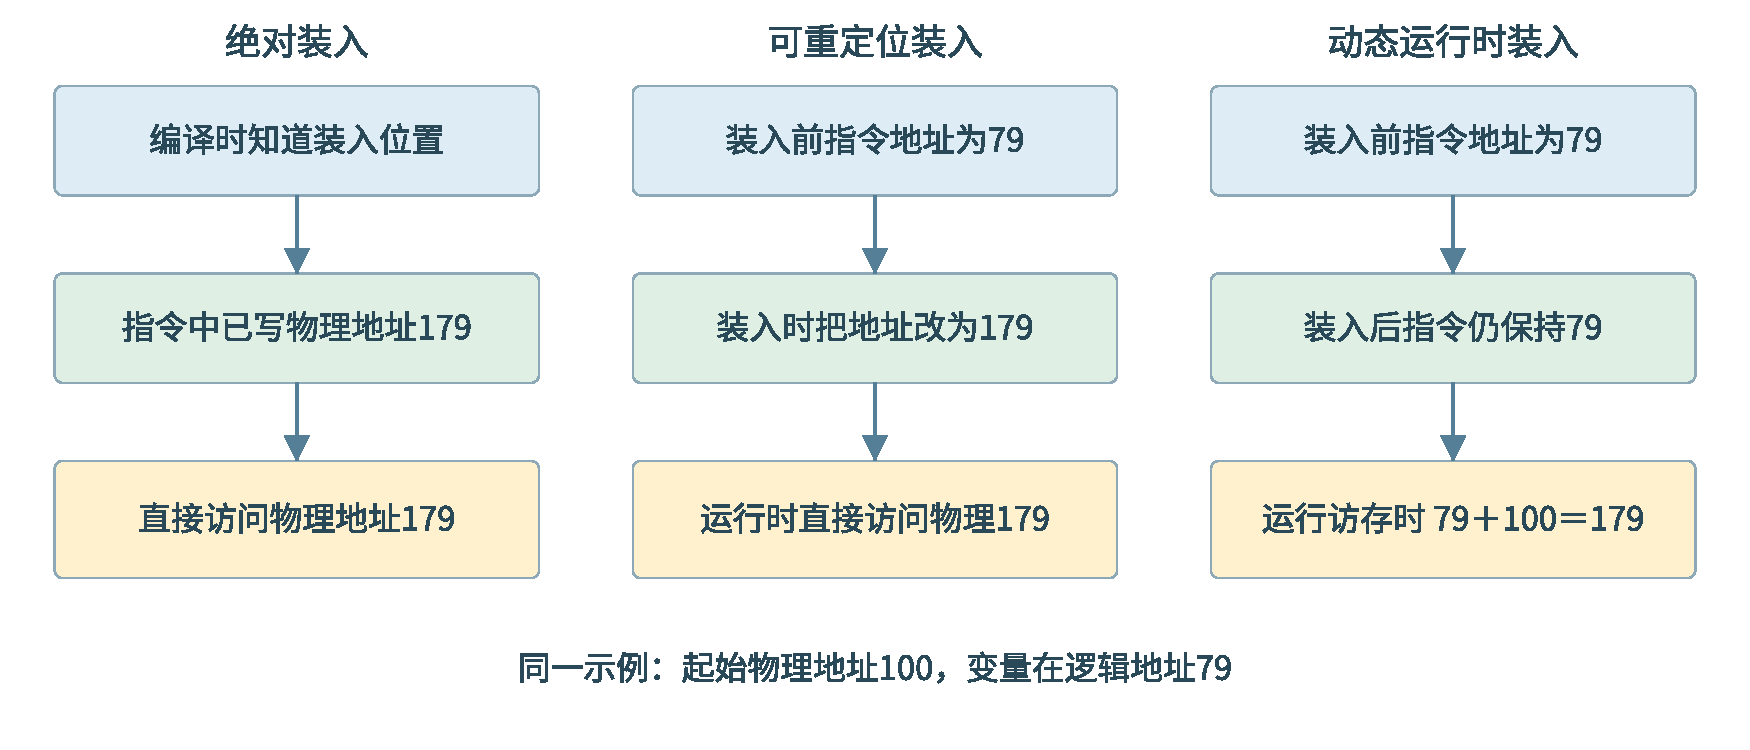
\includegraphics[width=\linewidth,height=125mm,keepaspectratio]{figures/OS03_loading_course.pdf}
\captionof{figure}{同一变量的三种装入：地址79与物理基址100}\label{os-fig-loading-course}
\end{minipage}\par\medskip

\end{wideblock}

地址保护的寄存器含义要与比较式一致。若基址为100，合法逻辑地址为0～179，界限寄存器保存最大合法逻辑地址179，则应检查\(0\le a\le179\)，物理地址为\(100+a\)；若界限保存长度180，则应检查\(0\le a<180\)。最大地址与长度相差1，属于两种字段定义，不能只凭``界限寄存器''这个名称选择比较符。

以上下限寄存器保护物理区域时，分别比较要访问的物理地址与100、279；采用重定位寄存器和界地址寄存器时，可先将逻辑地址与最大合法值179比较，再把合法的逻辑地址80加基址100，得到物理地址180。两种结构须分别看清所比较的地址及寄存器含义。

\begin{wideblock}

\par\medskip\noindent\begin{minipage}{\linewidth}
\centering
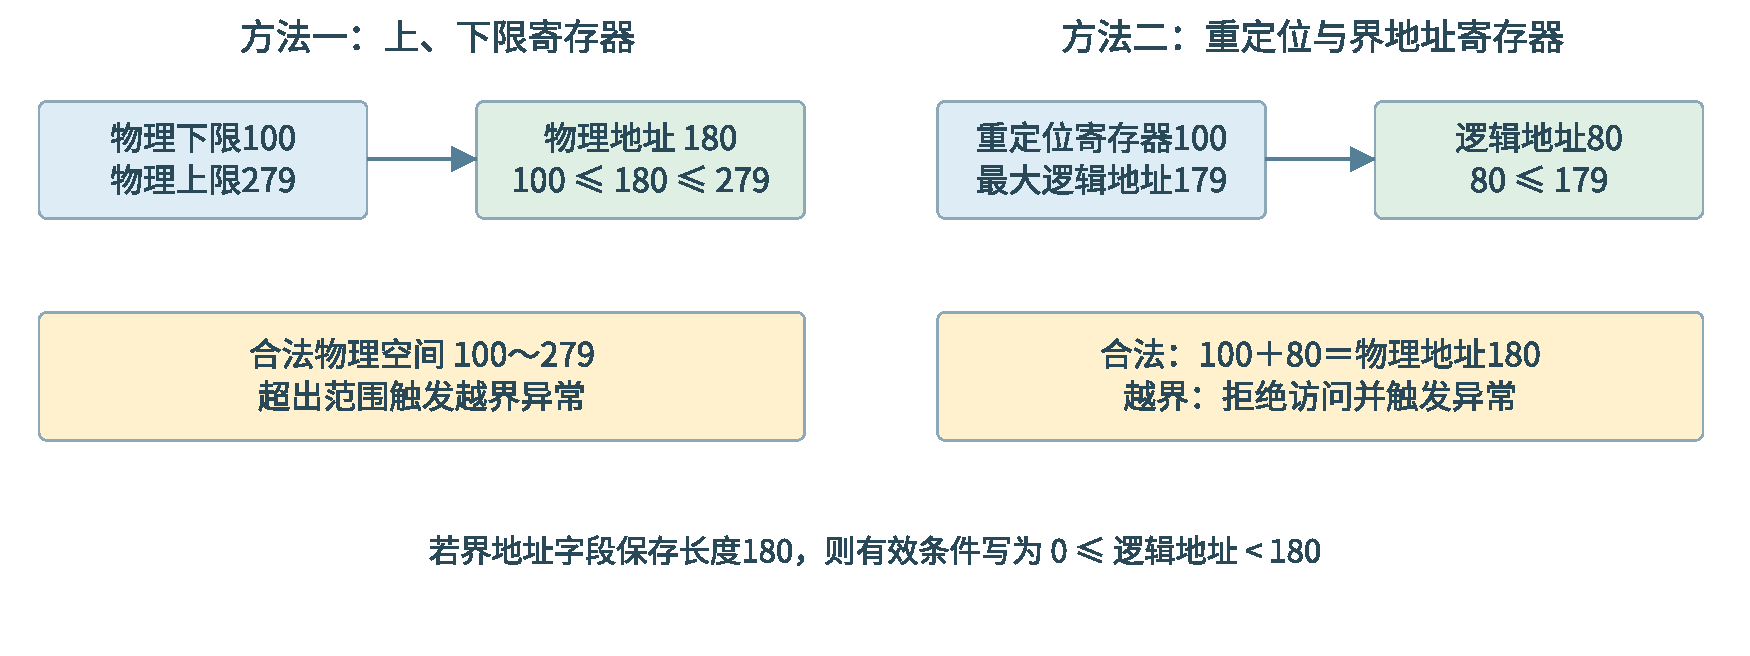
\includegraphics[width=\linewidth,height=125mm,keepaspectratio]{figures/OS03_protection_course.pdf}
\captionof{figure}{上下限保护与基址加界地址保护的比较流程}\label{os-fig-protection-course}
\end{minipage}\par\medskip

\end{wideblock}

进程的典型虚拟映像可含只读代码／数据、可读写静态数据、堆、共享库映射、栈及内核映射区域。代码中的宏常量可能在预处理后被替换，并不因此单独分配一个运行时对象；局部指针自身与\texttt{malloc}得到的堆对象仍要分别定位。具体地址分布、增长方向与是否保留内核映射，以题目平台为准。

\begin{wideblock}

\par\medskip\noindent\begin{minipage}{\linewidth}
\centering
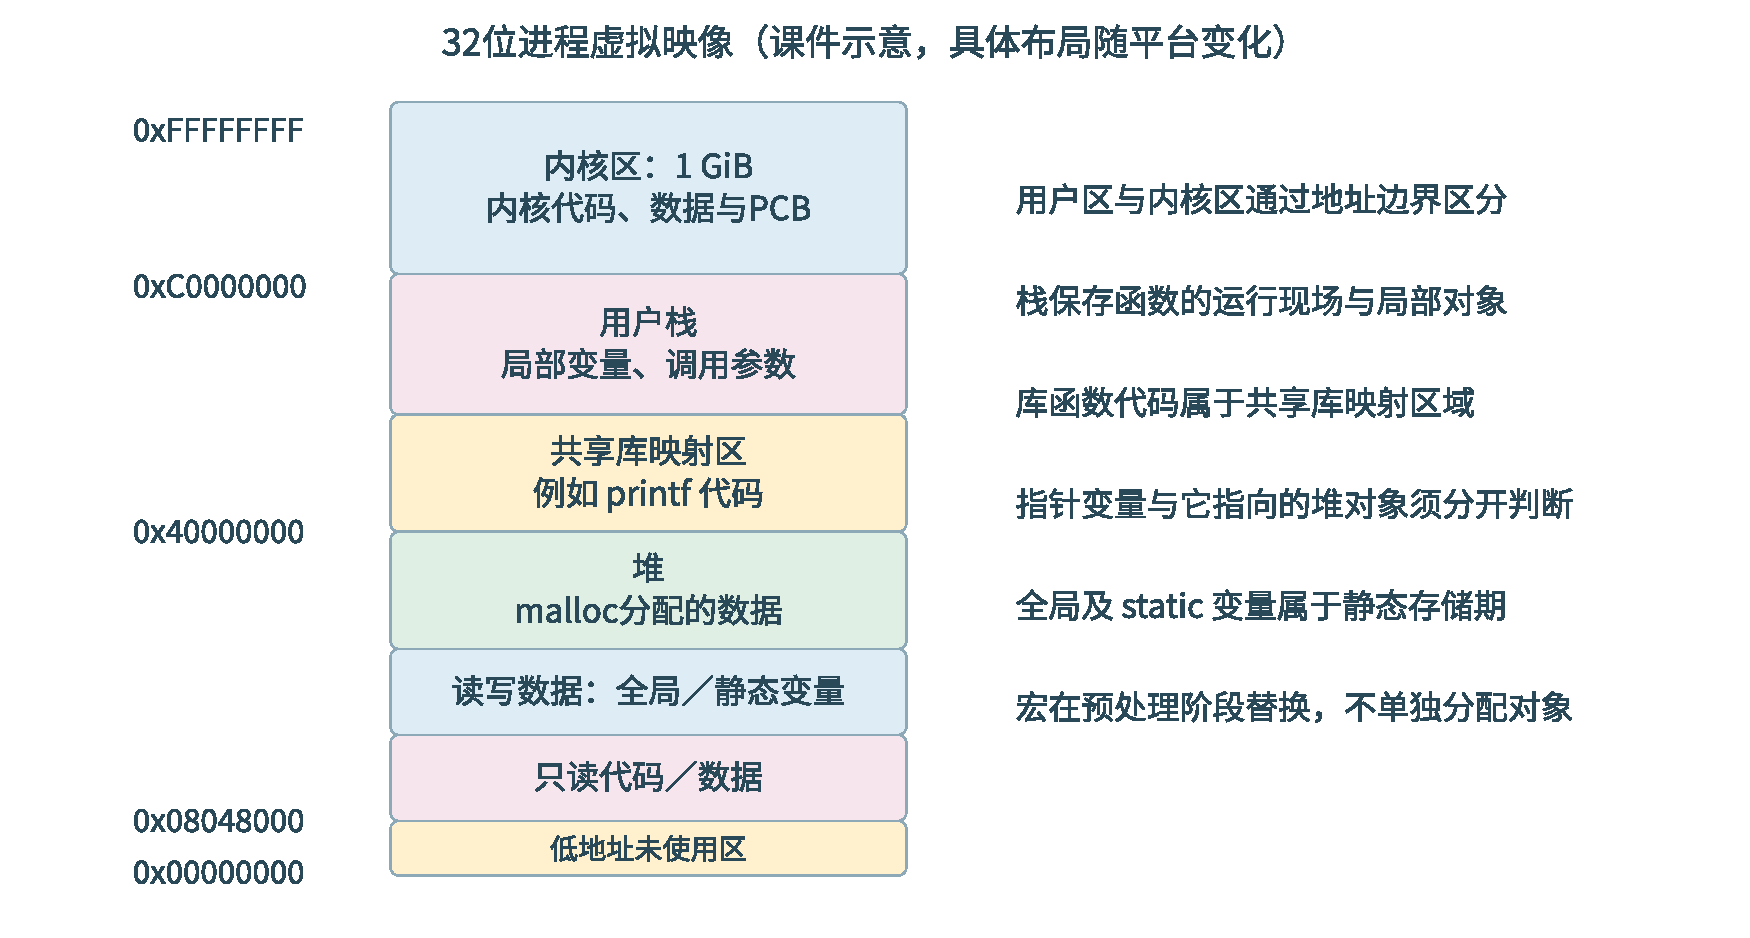
\includegraphics[width=\linewidth,height=125mm,keepaspectratio]{figures/OS03_process_image_course.pdf}
\captionof{figure}{32位进程虚拟映像的课件示例，标明用户栈、共享库、堆及代码数据区域}\label{os-fig-process-image-course}
\end{minipage}\par\medskip

\end{wideblock}

\section{共享、保护、分配和回收}\label{OS03-5-2}

分配决定哪些物理空间供谁使用，保护限制哪些操作合法，共享则允许多个映射指向同一内容。基址与界限可以保护连续区域；分页与分段通常在映射项中记录存在、读写、用户/内核等权限。一个地址有数值，不表示它属于合法映射；一个页面驻留内存，也不表示用户可以任意写入。

共享只读代码时，各进程的页表可以指向同一个物理页框，并禁止写入。共享可写数据则还需要同步。写时复制先把多个映射指向同一只读物理页，在某个进程需要写时触发受控异常，为写者分配并复制私有页，再更新映射；它与让所有写者始终修改同一共享页不同。

回收时必须维护使用计数、映射与空闲结构；若另一个进程仍在合法使用共享页，不能因为本进程退出就立即把页框分给无关对象。页表与 TLB 的映射变化也须保持一致，否则 TLB 中的过期转换可能继续生效，使访问落到已经回收或改变权限的内容上。

\subsection{例 3-1　页号可以不同，共享的页框必须相同}\label{OS03-ex5-1}

\begin{example}[配套例题]

【配套例题】 进程 R 和 S 共享数据 data。若 data 在两进程中的页号分别为 p1、p2，对应页框号分别为 f1、f2，下列叙述中，正确的是（　）。

A. p1、p2 一定相等，f1、f2 一定相等

B. p1、p2 一定相等，f1、f2 不一定相等

C. p1、p2 不一定相等，f1、f2 一定相等

D. p1、p2 不一定相等，f1、f2 不一定相等

\end{example}

\textbf{解析。} 两进程的虚拟布局可以不同，所以共享对象可以分别位于不同页号；题目所指的同一份共享数据在物理内存中是一份，对应页框号应相同。答案为 \textbf{C}。各自复制了一份内容相同的数据，不等于本题的共享映射。

\section{连续分配与动态分区：空闲总量不等于可分配块}\label{OS03-5-3}

单一连续分配把内存划分为系统区和一个用户区，不能有效支持多个驻留用户作业。固定分区预先划定若干区，每区容纳一个作业；作业小于分区时，分区内未用部分形成\textbf{内部碎片}。动态分区按请求划出连续区域，空闲洞可能被已分配区隔开，形成\textbf{外部碎片}：空闲总量够，仍可能没有一个足够大的连续洞。

\subsection{固定分区的划分与分区说明表}\label{OS03-fixed-partition-course}

固定分区可以等大，也可以不等大。等大分区易管理，适合多个大小相近的作业；大小不等可按常见作业规模划分多个小分区、适量中等分区和少量大分区，使不同作业更容易找到合适空间。两种情况每个分区同一时刻都只装入一道作业，程序太大而没有任何分区容得下时，不能把几个不连续的固定分区直接当成一块连续区。

\begin{wideblock}

\par\medskip\noindent\begin{minipage}{\linewidth}
\centering
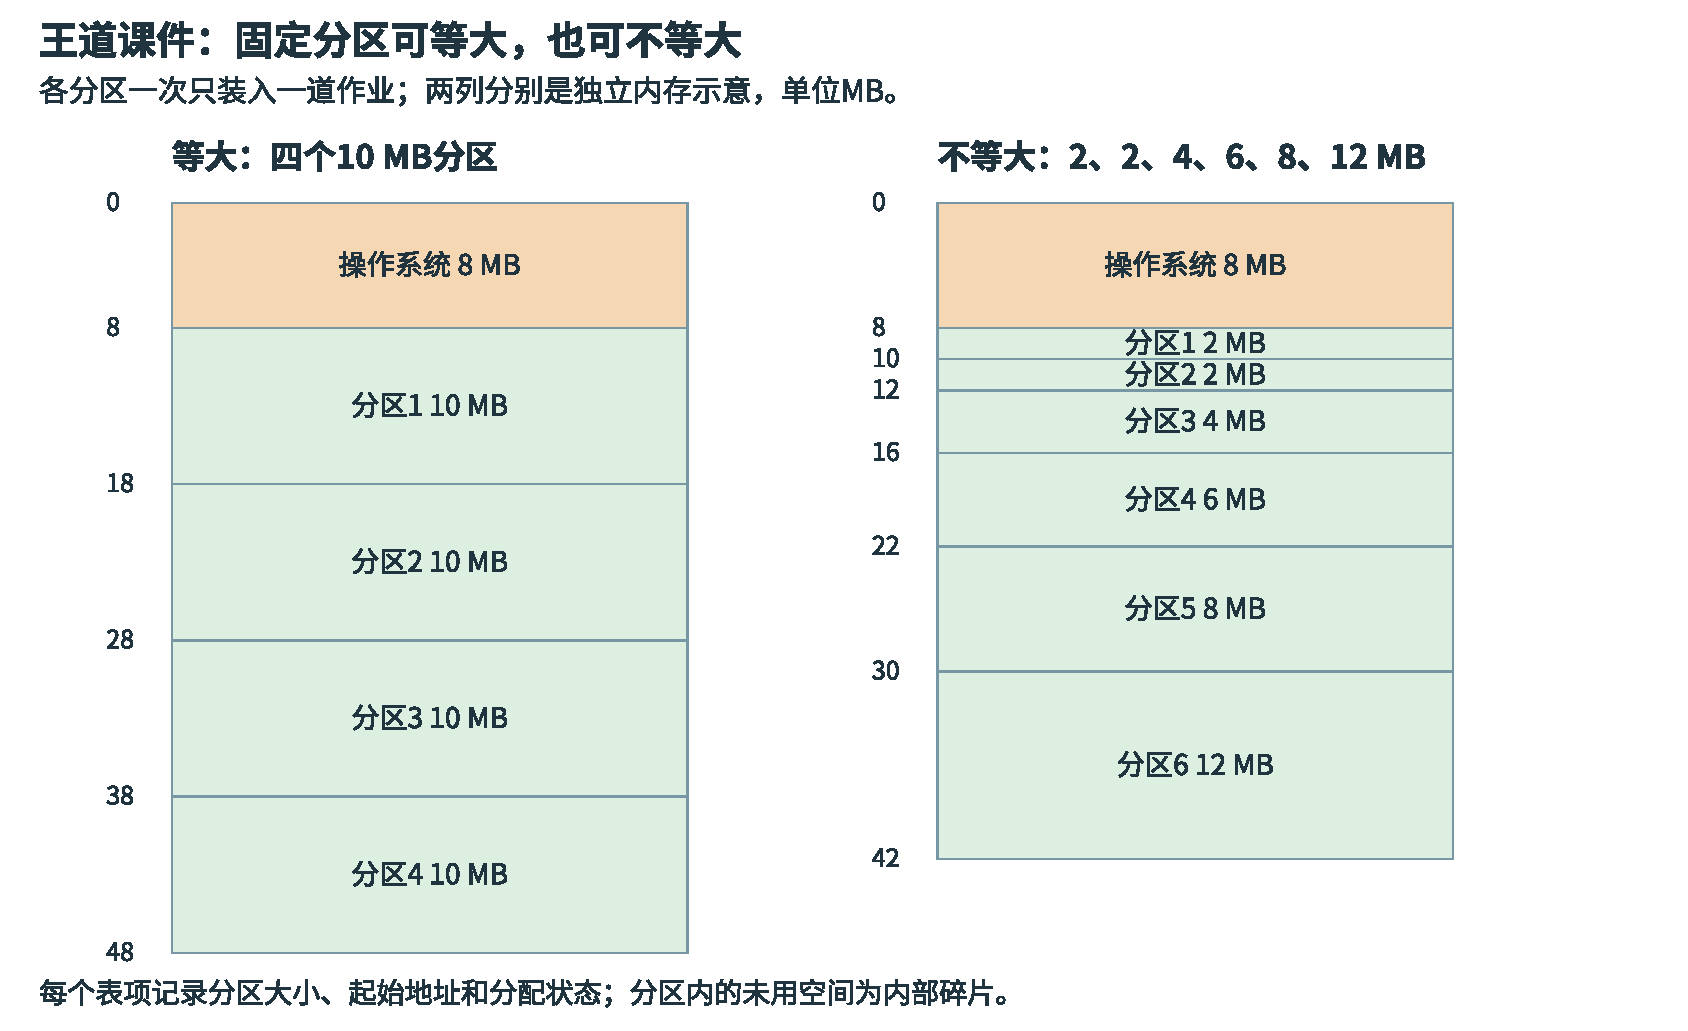
\includegraphics[width=\linewidth,height=125mm,keepaspectratio]{figures/OS03_fixed_partition_course.pdf}
\captionof{figure}{固定分区课件示例：系统区8 MB；等大分区每个10 MB，不等大分区依次2、2、4、6、8、12 MB}\label{os03-fixed-partition-figure}
\end{minipage}\par\medskip

\end{wideblock}

操作系统用分区说明表记录分区号、大小、起始地址及已分配状态；分配时检索可容纳作业的未分配分区，再把该表项改为已分配。课件示例表的前三项如下：

\begin{wideblock}\par\medskip\noindent\begin{minipage}{\linewidth}\fontsize{9.3}{12}\selectfont\begin{tabularx}{\linewidth}{@{}YYYY@{}}
\toprule\noalign{}
分区号 & 大小（MB） & 起始地址 & 状态 \\
\midrule\noalign{}


1 & 2 & 8 MB & 未分配 \\
2 & 2 & 10 MB & 未分配 \\
3 & 4 & 12 MB & 已分配 \\
\bottomrule\end{tabularx}
\end{minipage}\par\medskip\end{wideblock}

例如把1 MB作业装入一个2 MB分区，剩余1 MB仍属于该已分配分区，是\textbf{内部碎片}；它不是可独立分配的空闲分区。若题目要求计算碎片，需根据实际作业大小、分区选择和所规定的管理粒度逐一确定。

首次适应按地址顺序找第一个足够大的洞；循环首次适应从上次位置继续；最佳适应选择最小但够用的洞，常需按大小查找；最坏适应选择最大的洞。按课件的常见实现，首次适应与邻近适应将空闲链按地址递增排列，邻近适应可采用循环链并从上次检索结束处继续；最佳适应按容量递增，最坏适应按容量递减。首次适应常反复经过低地址的小洞，但也较可能保留高地址大洞；邻近适应分散检索，可能更早切分高地址大洞。最佳适应可能产生难利用的小碎片，最坏适应可能较快耗尽大洞；实际效果取决于请求序列与回收情况。算法只是在现有空闲区中选择一块，并不会把它们自动合并。最佳适应会留下很小的余量，``最接近请求''不保证长期整体利用率最好。

\subsection{课件实例：空闲链如何随分配变化}\label{OS03-course-partition-choices}

图中的前三组以同一组空闲区开始：大小20 MB、起始地址8；大小10 MB、起始地址32；大小4 MB、起始地址60。方框中的``大小 @ 起始地址''表示一段连续空闲区，按该算法维护的空闲链次序排列；分配从所选空闲区的低地址端切出。三个算法的进程请求大小以各自课件演示为准，不能把不同演示的请求混成同一组。

\begin{wideblock}

\par\medskip\noindent\begin{minipage}{\linewidth}
\centering
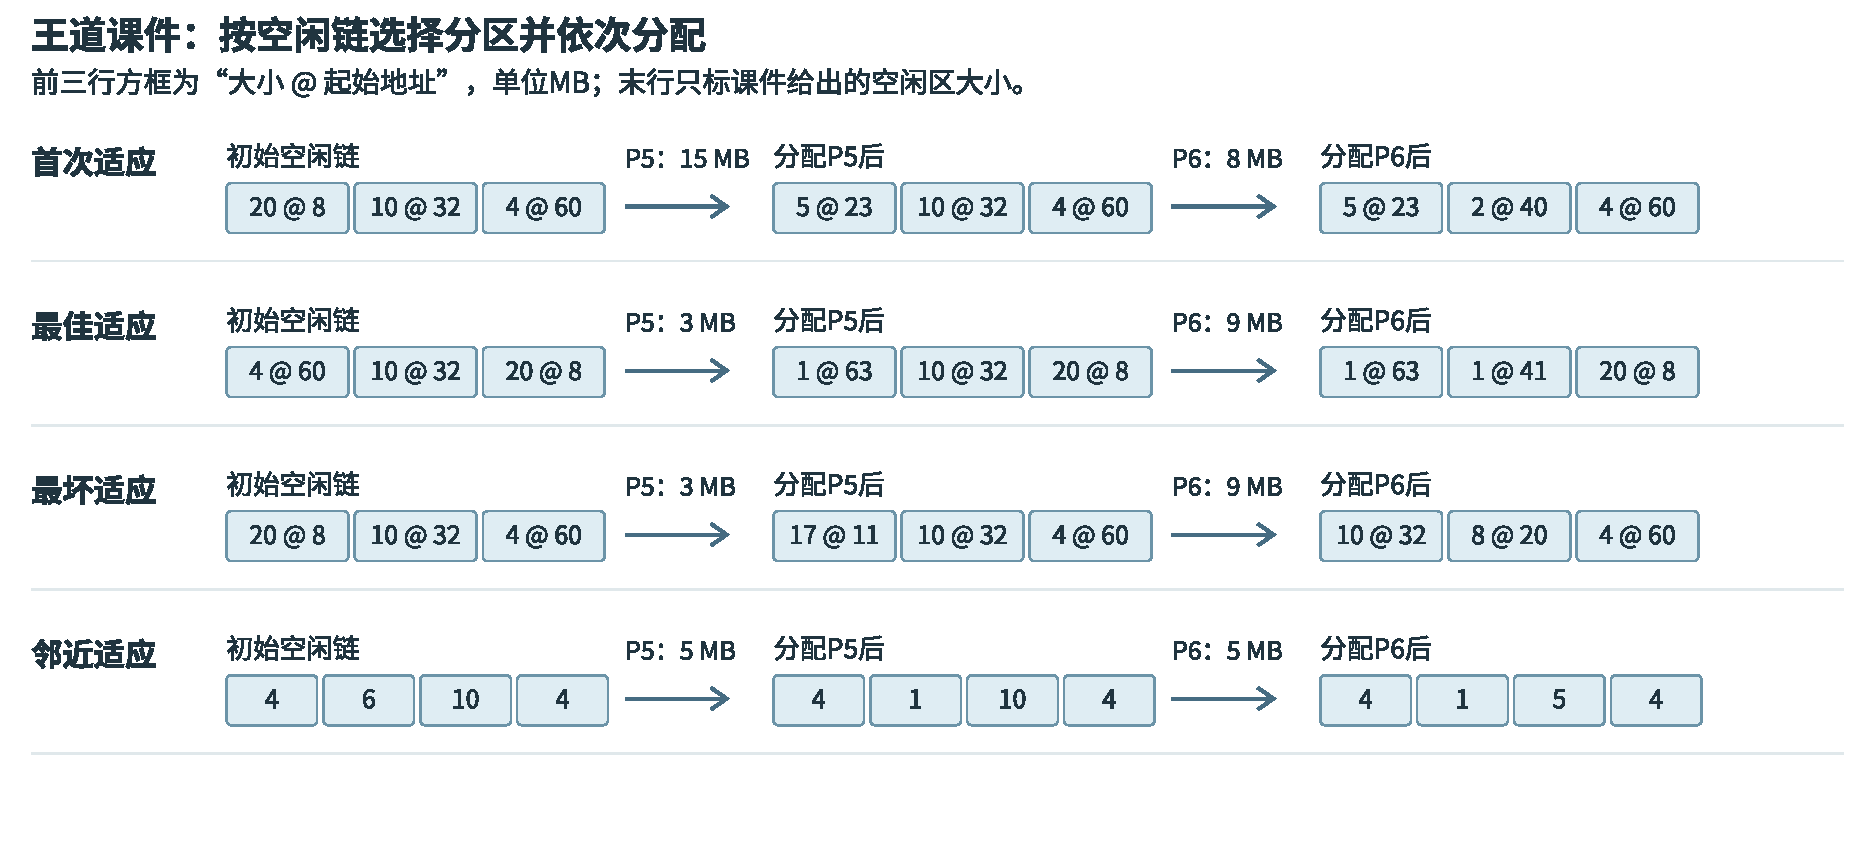
\includegraphics[width=\linewidth,height=125mm,keepaspectratio]{figures/OS03_partition_algorithms_course.pdf}
\captionof{figure}{四种动态分区分配算法的课件空闲链演示}\label{os03-partition-course}
\end{minipage}\par\medskip

\end{wideblock}

首次适应依地址递增：P5请求15 MB，从20 MB区切出后留下大小5、起始23的空闲区；P6请求8 MB，5 MB不足，再从起始32的10 MB区切出，留下大小2、起始40。最佳适应按容量递增：P5的3 MB先选起始60的4 MB区，P6的9 MB再选起始32的10 MB区，分别留下两个1 MB碎片。最坏适应按容量递减：两个请求先后从原20 MB区切出，余区依次为17 MB和8 MB；第二次分配后，空闲链须重新按大小排列，10 MB排在8 MB之前。

邻近适应的课件演示使用地址递增的循环空闲链，大小依次为4、6、10、4 MB。P5的5 MB由6 MB区分出，P6的5 MB由10 MB区分出，余区大小依次为4、1、5、4 MB。它从上次查找结束处继续，查至链尾仍未找到时回到链头；具体起始指针位置是确定下一次结果所必需的状态。四组图展示的是课件演示过程，算法长期表现还取决于请求与回收序列。

释放分区时检查物理地址是否相邻：只与前洞相邻则合并前洞，只与后洞相邻则合并后洞，前后都邻接则合并三块。在按大小排序的空闲区表中，相邻表项未必在物理地址上相邻。紧凑通过搬移已分配内容把分散空洞合成大洞，需要可重定位支持和搬移成本，这与释放时合并相邻空闲区不是一回事。

\subsection{例 3-2　最佳适应每次都重新比较当前空闲区}\label{OS03-ex5-2}

\begin{example}[配套例题]

【配套例题】 某基于动态分区存储管理的计算机，主存容量为 55 MB（初始为空闲），采用最佳适配算法。分配和释放顺序为：分配 15 MB，分配 30 MB，释放 15 MB，分配 8 MB，分配 6 MB。此时最大空闲分区为（　）。

A. 7 MB　　B. 9 MB\\
C. 10 MB　　D. 15 MB

\end{example}

\textbf{解析。} 前两次分配后剩余 10 MB；释放最初的 15 MB 后，有两个不相邻的洞：15 MB 和 10 MB。分配 8 MB 时，最佳适应从 10 MB 中切出，留下 2 MB；分配 6 MB 时，2 MB 不够，只能从 15 MB 中切出，留下 9 MB。因此两个洞为 9 MB、2 MB，最大 9 MB，答案为 \textbf{B}。

\begin{wideblock}

\par\medskip\noindent\begin{minipage}{\linewidth}\fontsize{9.3}{12}\selectfont\begin{tabularx}{\linewidth}{@{}YY@{}}
\toprule\noalign{}
操作后 & 当前空闲分区大小 \\
\midrule\noalign{}


分配 15 MB & 40 MB \\
再分配 30 MB & 10 MB \\
释放最初的 15 MB & 15 MB、10 MB \\
分配 8 MB & 15 MB、2 MB \\
分配 6 MB & 9 MB、2 MB \\
\bottomrule\end{tabularx}
\end{minipage}\par\medskip

\end{wideblock}

这里不能先把 15 与 10 相加，因为中间仍有占用区；也不能在分配 8 MB 时沿用首次适应的地址顺序。

\subsection{空闲区表与回收时的四种合并}\label{OS03-partition-recovery}

动态分区用空闲区表或空闲区链记录起始地址和长度。分配时选中一块，若只使用其一部分，就更新剩余区间；释放时根据物理地址邻接关系合并，避免把已经连成一片的空闲区误保留为多个洞。

\textbf{课件中的分配更新。} 空闲表含起始8、大小20 MB，起始32、大小10 MB，以及起始60、大小4 MB的三个表项。给P5分配4 MB时，若选前20 MB区并从低地址切出，分配区为\([8,12)\)，把该表项改为起始12、大小16 MB；若选末尾4 MB区，则\([60,64)\)恰好用完，应删除对应空闲表项。其他空闲表项保持原值。两种情况是从同一初始状态出发的独立演示，具体选哪一块由题设采用的分配算法决定。

\begin{wideblock}

\par\medskip\noindent\begin{minipage}{\linewidth}
\centering
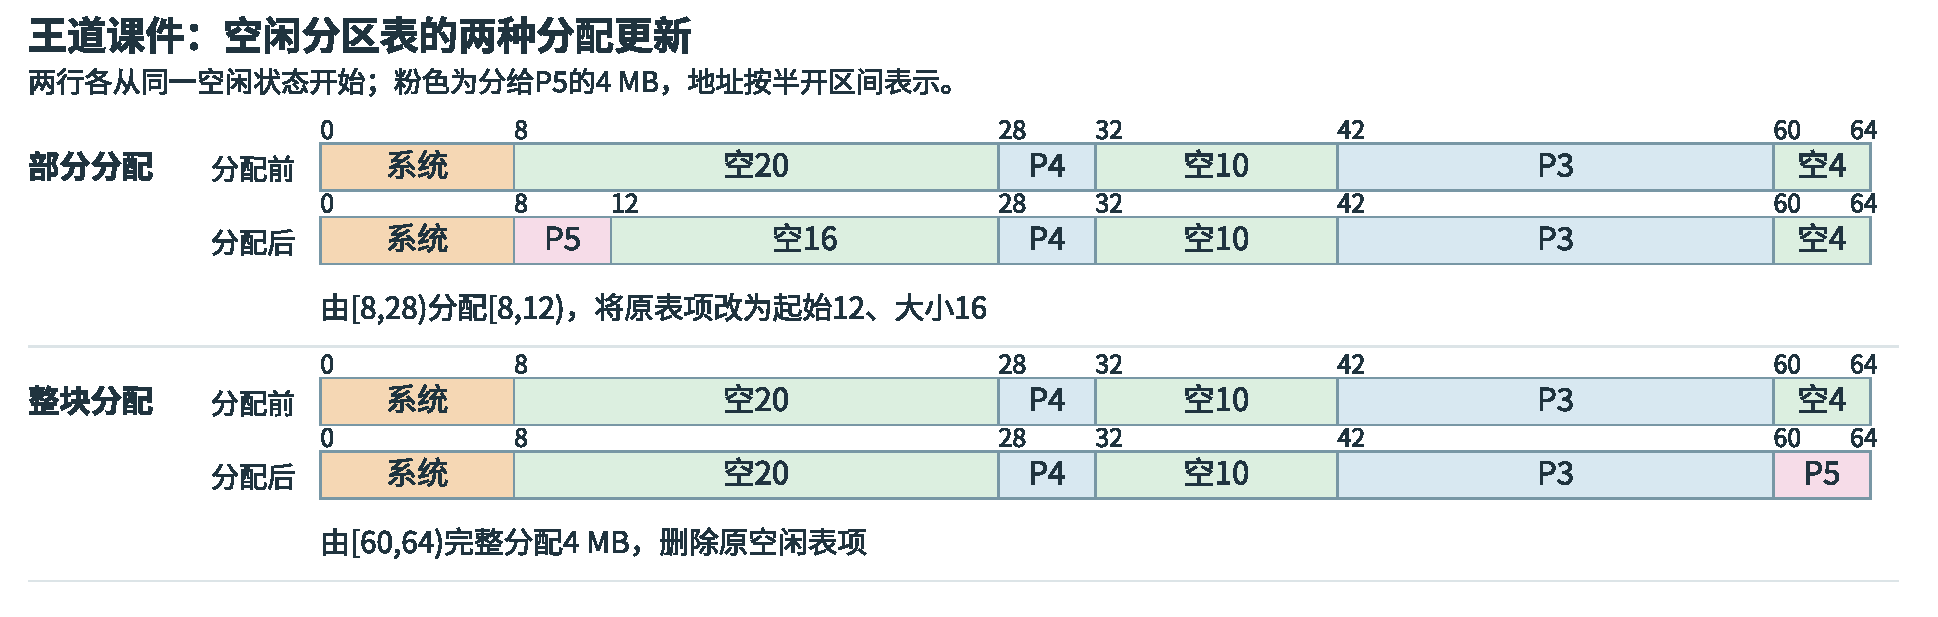
\includegraphics[width=\linewidth,height=125mm,keepaspectratio]{figures/OS03_partition_allocation_course.pdf}
\captionof{figure}{空闲分区表中切出一部分与恰好用完整块的两种更新}\label{os03-partition-allocation-figure}
\end{minipage}\par\medskip

\end{wideblock}

课件64 MB模型中系统区占前8 MB，空闲区可为\([8,28)\)、\([32,42)\)、\([60,64)\)，长度分别20、10、4 MB；区间右端不包含。若释放\([28,32)\)的4 MB区域，它同时连接前后两个洞，应合成\([8,42)\)，长度34 MB，并保留\([60,64)\)。

\begin{wideblock}

\par\medskip\noindent\begin{minipage}{\linewidth}
\centering
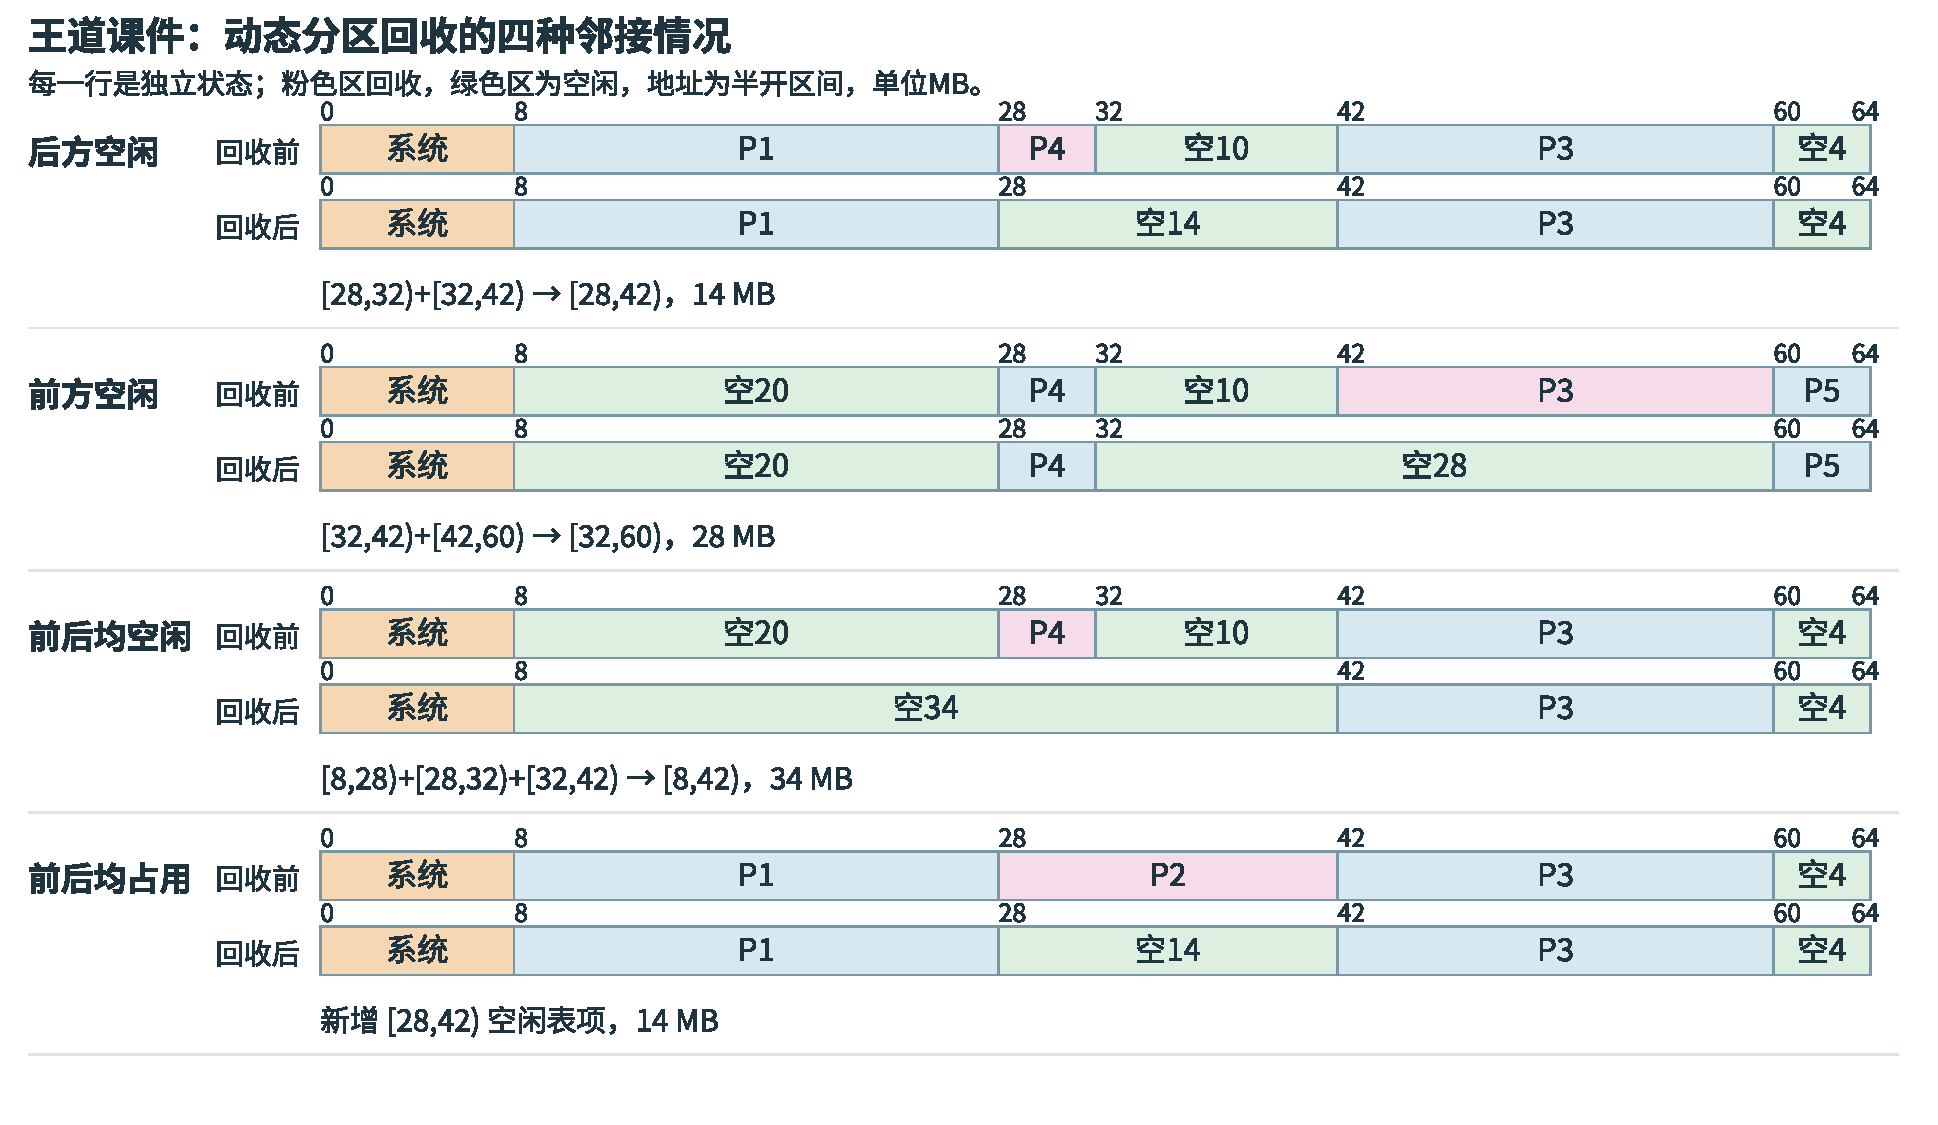
\includegraphics[width=\linewidth,height=125mm,keepaspectratio]{figures/OS03_partition_reclaim_course.pdf}
\captionof{figure}{课件四种回收情况：前后空闲区分别相邻、两侧都相邻或都不相邻}\label{os-fig-partition-merge}
\end{minipage}\par\medskip

\end{wideblock}

图中四行分别是独立的课件状态，并非连续的四次回收：只与后方相邻时，释放\([28,32)\)并与\([32,42)\)合成\([28,42)\)，长度14 MB；只与前方相邻时，释放\([42,60)\)并与\([32,42)\)合成\([32,60)\)，长度28 MB。前后都相邻时合成\([8,42)\)、长度34 MB；前后均不空闲时，释放\([28,42)\)后新增长度14 MB的空闲表项。

\par\medskip\noindent\begin{minipage}{\linewidth}\fontsize{9.3}{12}\selectfont\begin{tabularx}{\linewidth}{@{}YY@{}}
\toprule\noalign{}
回收区与已有空闲区关系 & 更新方法 \\
\midrule\noalign{}


前后均不相邻 & 新建空闲表项 \\
只与前方空闲区相邻 & 前方表项长度增加 \\
只与后方空闲区相邻 & 后方表项起址前移、长度增加 \\
前后都有相邻空闲区 & 三段合并，保留一个表项并删除多余表项 \\
\bottomrule\end{tabularx}
\end{minipage}\par\medskip

首次适应按地址递增检索；最佳适应按足够容纳请求的最小长度选择；最坏适应选最大长度；邻近适应从上次检索位置继续。表若按容量排列，回收后可能重新排序，因此``表项挨在一起''不是判断物理相邻的证据。

\subsection{覆盖结构的容量计算}\label{OS03-overlay-example}

课件覆盖模型含主模块A为8 KB，B、C分别8、10 KB，D、E、F分别12、4、10 KB。把A放入固定区，让B与C共享10 KB覆盖区、D/E/F共享12 KB覆盖区，则这一安排需要\(8+10+12=30\) KB，而六模块长度之和为52 KB。

\begin{wideblock}

\par\medskip\noindent\begin{minipage}{\linewidth}
\centering
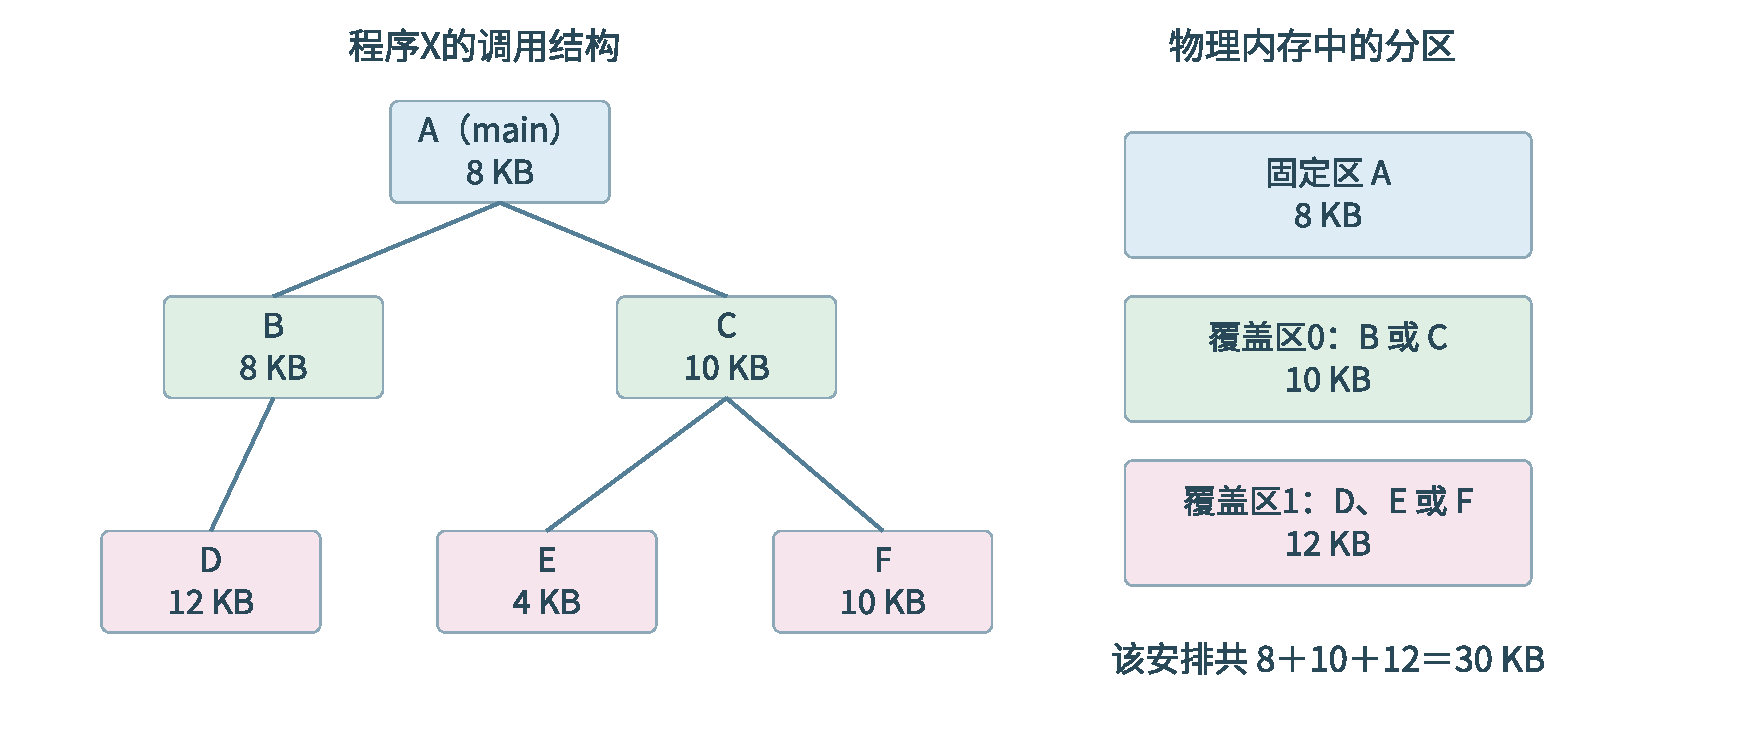
\includegraphics[width=\linewidth,height=125mm,keepaspectratio]{figures/OS03_overlay_course.pdf}
\captionof{figure}{A调用B、C，B调用D，C调用E、F；按调用结构划分固定区与两个覆盖区}\label{os-fig-overlay-course}
\end{minipage}\par\medskip

\end{wideblock}

该安排依赖模块调用关系，必须保证共享覆盖区内的模块不会同时需要保留有效执行内容。30 KB是这份覆盖安排的容量，不是在任意调用、递归或返回约束下自动成立的全局最小值。覆盖通常要求程序员提供覆盖结构；交换和请求分页由操作系统按其管理策略处理，透明程度不同。

\section{分页：页号查表，偏移不变}\label{OS03-5-4}

\textbf{分页}把虚拟地址空间划成固定大小的页，把物理内存划成同样大小的页框，页可以装入不相邻的页框。页表记录虚拟页到物理页框的映射。分页不再要求整个进程连续分配，从而消除了连续分配造成的外部碎片，但进程最后一页可能未用满，仍有内部碎片；页表也占空间。

页大小 \(P=2^d\) B，虚拟地址 \(a\) 分解为

\[p=\left\lfloor\frac aP\right\rfloor,\qquad w=a\bmod P.\]

按除法与取余的抽象示例，即使页长设为50 B，逻辑地址110仍可分解为页号 \(\lfloor110/50\rfloor=2\)、偏移 \(110\bmod50=10\)。该算例说明分解方法；常见硬件采用2的幂大小，是为了直接用位字段完成分解。

查得页框号 \(f\) 后，物理地址为 \(fP+w\)。低 \(d\) 位偏移不变，高位的虚拟页号被页框号替换。页表项本身也存放在物理内存中，它的地址是另一个物理地址：单级线性页表基址为 \(PTBR\)、每项 \(e\) B 时，页 \(p\) 的项地址为 \(PTBR+pe\)。不要把页表项地址当成最终数据地址。

\textbf{课件位拼接例。} 页大小4 KiB，逻辑地址4097分解为页号1、页内偏移1；若页1映射到页框9，则物理地址为 \(9\times4096+1=36865\)。页框号9的二进制为 \(1001_2\)，将其与12位偏移 \(000000000001_2\) 拼接，得到 \(1001\,000000000001_2=9001_H=36865\)。拼接时偏移必须保留完整的12位。

配套分页例中，页大小 1 KB，逻辑地址 0A6FH，页 0、1、2、3 分别映射页框 3、7、11、10。\(0A6F_H=2\times400_H+26F_H\)，故页号为 2，偏移 26FH；查到页框 11，即 BH，物理地址为 \(B\times400_H+26F_H=2E6F_H\)。偏移字段跨越十六进制数位，不能简单截取最后两位或三位。

页表项至少要能表示页框号，通常还包含存在、保护、访问和修改等信息。虚拟地址宽度决定潜在页数，物理地址宽度决定页框号所需位数；两者分别进入``页表多少项''和``每项至少多宽''的计算。

\subsection{基本地址变换的完整检查链}\label{OS03-page-translation}

页表寄存器保存页表起始地址和表长等信息；进程未运行时，相关环境可保存在PCB中，切换时由内核恢复。设页大小\(L\)、页表基址\(F\)、表长\(M\)项、每项\(e\)字节，地址\(A\)对应\(p=\lfloor A/L\rfloor\)、\(w=A\bmod L\)：

\begin{enumerate}
\def\labelenumi{\arabic{enumi}.}
\tightlist
\item
  先检查\(0\le p<M\)，等于表长时已经越界。
\item
  在紧密连续存放的单级页表中读取\(F+pe\)处的表项，得到页框号\(b\)及权限等。
\item
  确认本次访问合法后，形成物理地址\(E=bL+w\)，再访问目标单元。
\end{enumerate}

\par\medskip\noindent\begin{minipage}{\linewidth}
\centering
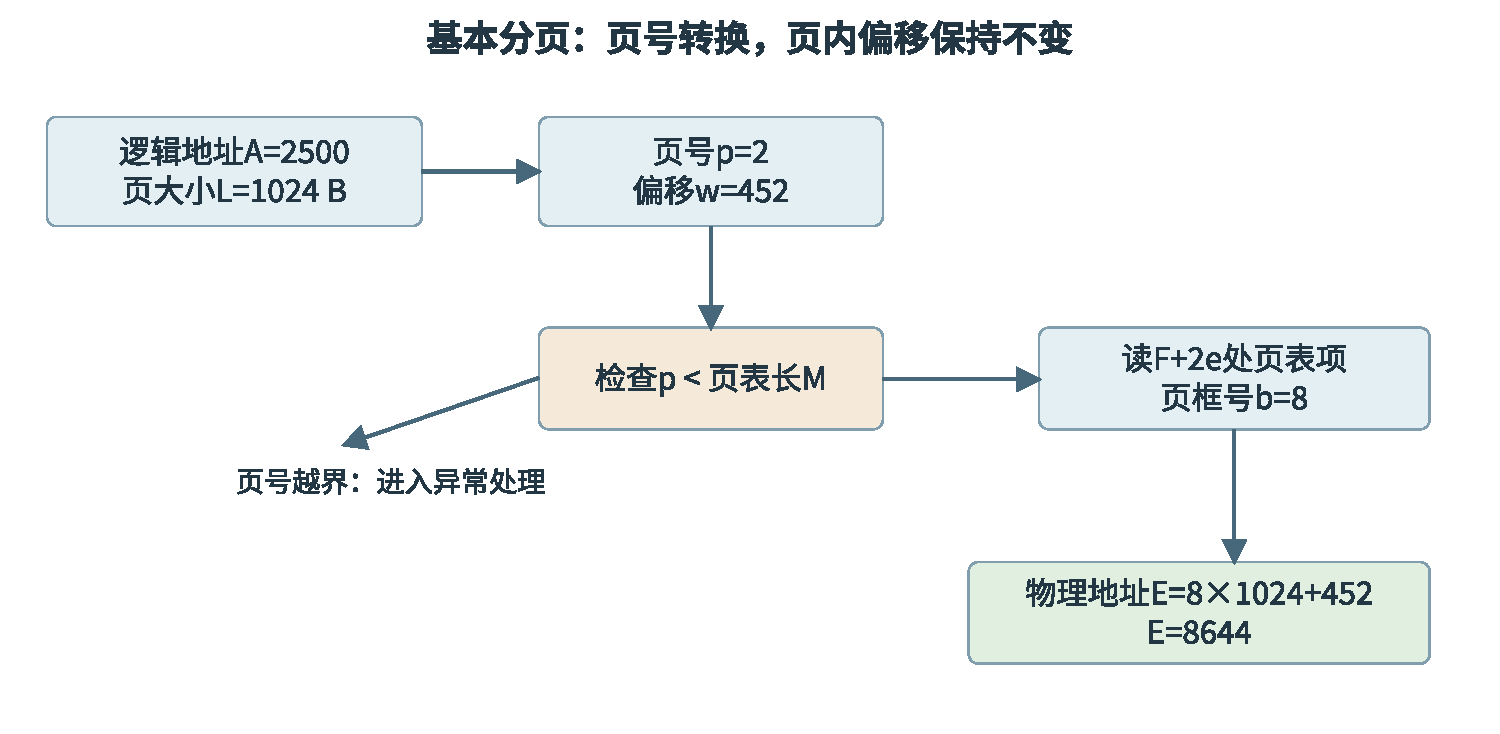
\includegraphics[width=\linewidth,height=125mm,keepaspectratio]{figures/OS_page_translation.pdf}
\captionof{figure}{逻辑地址分解、范围检查、页表访问和目标访问是不同步骤}\label{os-fig-page-translation}
\end{minipage}\par\medskip

课件十进制例中\(L=1024\) B、\(A=2500\)，故\(p=2,w=452\)；页2映射到页框8，物理地址为\(8\times1024+452=8644\)。页内偏移始终为452，不能在最后一步误换为425。页表项地址和最终数据地址则各自按对应公式计算。

\subsection{页表项位宽、对齐与装表空间}\label{OS03-pte-size}

若可寻址物理内存为4 GiB、页大小4 KiB，共有\(2^{20}\)个页框，单是页框号就需20位。向上按字节取整至少3 B；还需容纳权限、存在、访问、修改等字段，实际表项可能更大。

若每项4 B，一页可放1024项，表项边界与页边界整齐对应。若每项3 B且表项不得跨页，一页最多1365项，并有1 B尾部空隙；跨到下一页时，项地址还须计入该布局的空隙。公式\(F+pe\)采用的是紧密线性布局，不能同时假定每页留空隙又照用同一地址式。

页表总项数、每项长度、一个页面大小分别描述``映射多少页''``一项占多大''和``映射单位多大''，三者不能互换。多级页表的扇出计算也应先确认每张下级页表是否限定占一页。

\section{TLB 与多级页表：空间与时间分别计算}\label{OS03-5-5}

\subsection{多级页表为什么可以节省空间}\label{OS03-auto-1}

若虚拟页很多，单级页表需要大量表项，即使大部分虚拟区间根本没有使用。多级页表先用高层目录找到所需下级页表，仅为实际使用区域建立相应下级表；各下级表可以分别放置，不需要一块能容纳整张大页表的连续内存。

多级页表不能减少``一个最终映射项本身需要的位数''，也不保证为一个占满全部虚拟空间的进程节省总空间；全展开时还增加目录开销。它的收益主要体现在稀疏地址空间和分级分配上，代价是未命中转换缓存时要多次查表。

\subsection{王道课件：逐级转换与级数计算}\label{OS03-course-twolevel}

\textbf{逐级转换。} 某二级分页系统的地址依次由10位一级页号、10位二级页号和12位页内偏移构成。逻辑地址为 \texttt{(\allowbreak{}0000000000,\allowbreak{}0000000001,\allowbreak{}111111111111)\allowbreak{}}。一级页号为0，二级页号为1，页内偏移为 \(2^{12}-1=4095\)。按题目页表从目录项0取得下级页表，再查其第1项，得到页框号4；最终物理地址为 \(4\times4096+4095=20479\)。逐级查询得到的页框号才用于末步计算，不能把一级目录项中的下级页表页框号当作目标数据页框号。

\begin{wideblock}

\par\medskip\noindent\begin{minipage}{\linewidth}
\centering
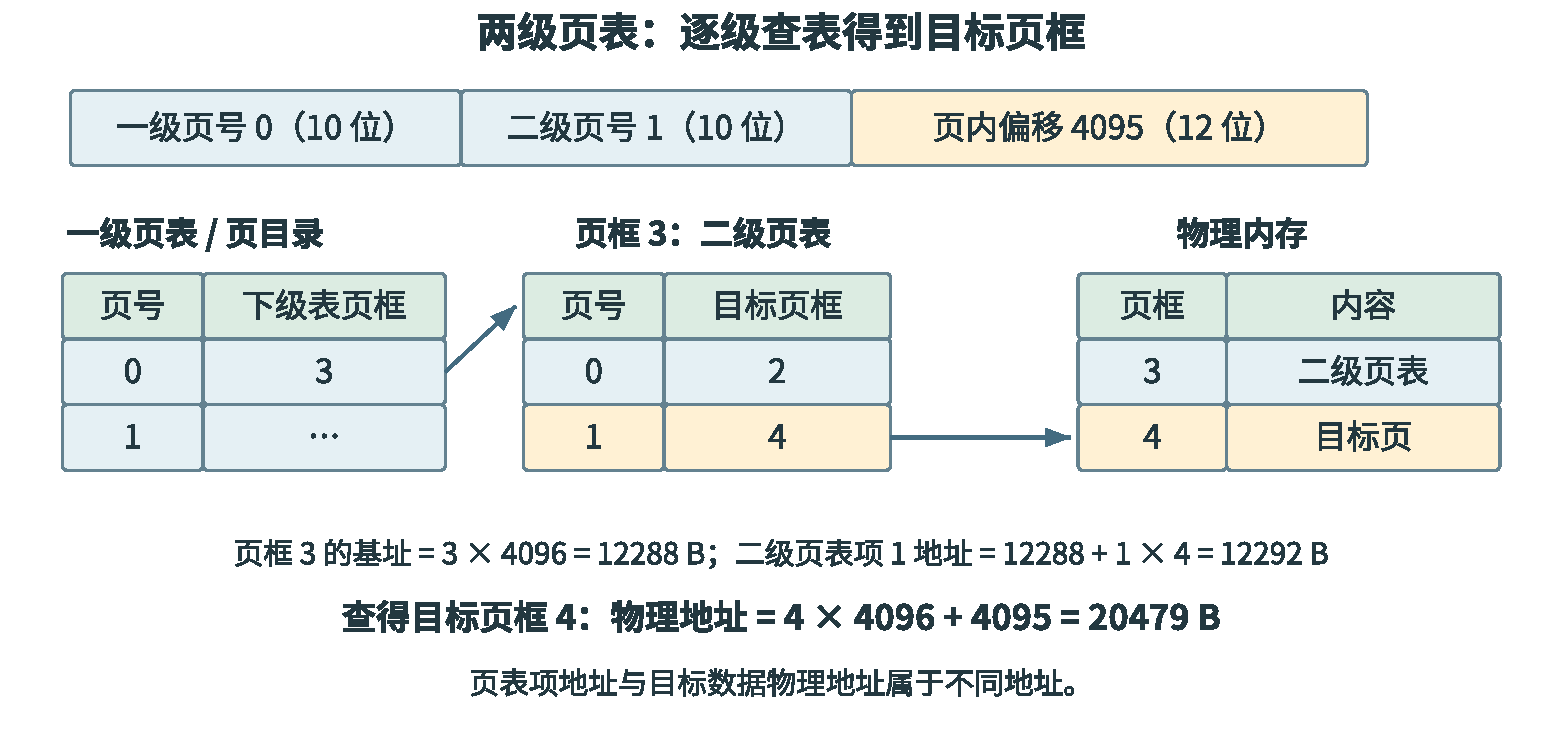
\includegraphics[width=\linewidth,height=125mm,keepaspectratio]{figures/OS03_twolevel_course.pdf}
\captionof{figure}{10／10／12位地址依次查页目录、二级页表并形成物理地址}\label{os03-twolevel-course}
\end{minipage}\par\medskip

\end{wideblock}

\textbf{需要多少级页表。} 逻辑地址40位，按字节编址，页面4 KB，页表项4 B，且每张页表最多占一个页面。页内偏移为12位，虚拟页号为 \(40-12=28\) 位；每页最多存放 \(4096/4=1024=2^{10}\) 个页表项，每级最多覆盖10位页号。因此至少需要 \(\lceil28/10\rceil=3\) 级，顶层不必使用满10位。这里的``至少3级''依赖每张表最多占一页和题目给出的页表项大小；页表可跨页时须重新确定分级方案。

\subsection{例 3-3　一张下级表能覆盖多少页}\label{OS03-ex5-3}

\begin{example}[配套例题]

【配套例题】 某计算机采用二级页表，按字节编址，页大小为 \(2^{10}\) B，页表项大小为 2 B，逻辑地址依次由页目录号、页号、页内偏移量组成。逻辑地址空间大小为 \(2^{16}\) 页，表示整个逻辑地址空间的页目录表至少包含多少表项？

A. 64　　B. 128\\
C. 256　　D. 512

\end{example}

\textbf{解析。} 一张按页存放的下级页表能容纳 \(2^{10}/2=2^9\) 项，故能映射 \(2^9\) 个虚拟页。要覆盖 \(2^{16}\) 页，需要 \(2^{16}/2^9=2^7=128\) 张下级表，也就是至少 128 个目录项，答案为 \textbf{B}。相应字段为目录 7 位、页号 9 位、偏移 10 位；``逻辑空间 \(2^{16}\) 页''不是 16 位字节地址，而是 16 位虚拟页号。

\subsection{例 3-4　10 位字段不能按十六进制整位截断}\label{OS03-ex5-4}

{\tcbset{SNbase/.append style={breakable=false}}\begin{example}[配套例题]

【配套例题】 某计算机主存按字节编址，二级分页地址结构依次为页目录号 10 位、页号 10 位、页内偏移 12 位。虚拟地址 2050 1225H 对应的页目录号、页号分别是（　）。

A. 081H、101H　　B. 081H、401H

C. 201H、101H　　D. 201H、401H

\par\medskip\noindent\begin{minipage}{\linewidth}
\centering
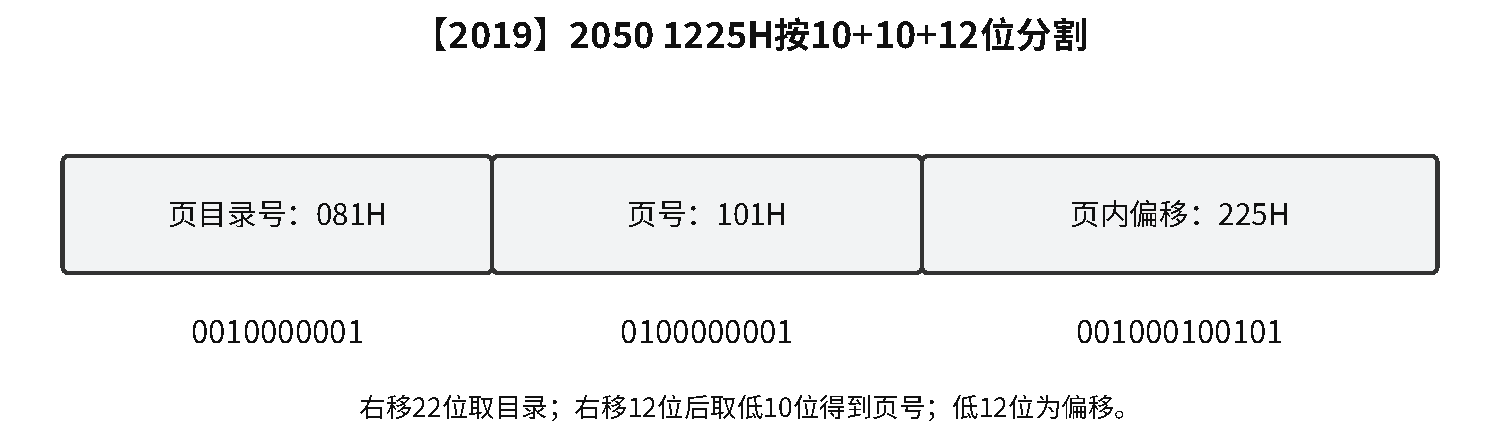
\includegraphics[width=\linewidth,height=125mm,keepaspectratio]{figures/OS_address_fields.pdf}
\captionof{figure}{先按二进制位宽分割，再将每一段单独转为十六进制}\label{os-fig-address}
\end{minipage}\par\medskip

\end{example}}

\textbf{解析。} 偏移为低 12 位 225H。目录号为地址右移 22 位，得 081H；下级页号为地址右移 12 位后取低 10 位，得 101H。答案为 \textbf{A}。若先把``205''当成某个字段，就把十六进制的 4 位分组误当成题设的 10 位字段。

\subsection{TLB 缓存的是转换，不是文件内容}\label{OS03-auto-2}

\textbf{快表 TLB}缓存近期地址转换及相关权限信息。命中时直接得到页框和权限；未命中时遍历页表，找到有效映射后可填入 TLB。TLB 未命中只说明转换不在该缓存，页面仍可能在内存；页表项表明合法页面不驻留才可能引发缺页。数据 Cache 缓存的则是实际数据，不能把 TLB 命中当成数据已经在 Cache。

\textbf{课件中的一种状态更新策略。} 访问命中时可先更新快表中的访问状态，写操作还需更新修改状态；移除该快表项前再把更新的状态写回内存页表，以减少频繁更新慢表带来的访存。页面置换和映射失效处理必须取得一致的状态。不同硬件和系统的状态更新策略可能不同，题目有明确规定时按题设处理。

\begin{wideblock}

\par\medskip\noindent\begin{minipage}{\linewidth}
\centering
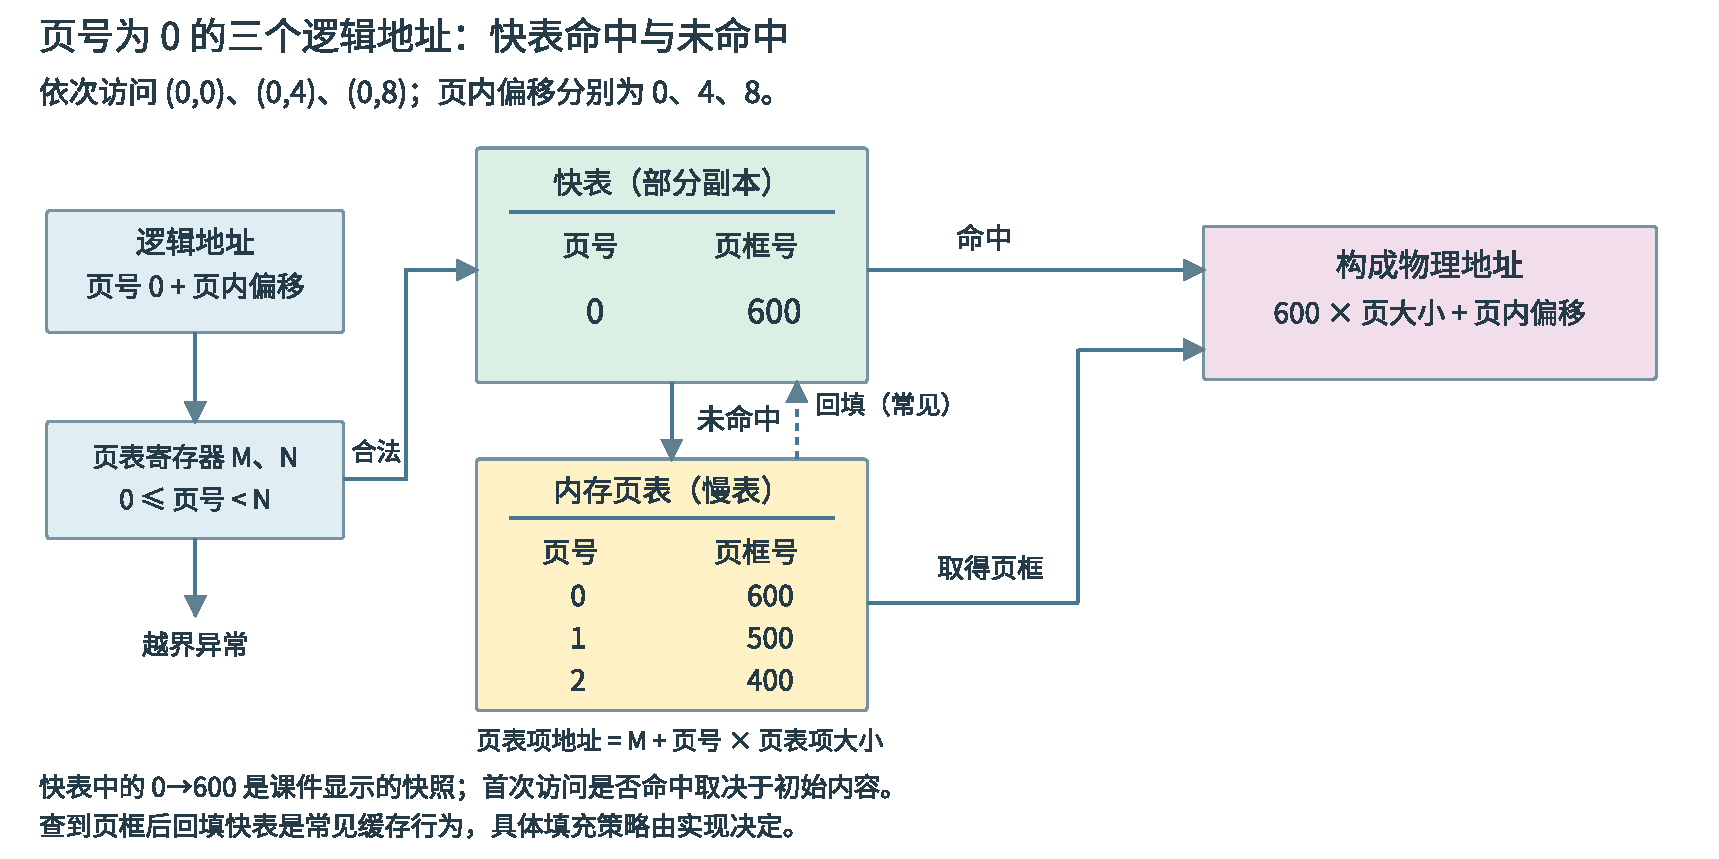
\includegraphics[width=\linewidth,height=125mm,keepaspectratio]{figures/OS03_tlb_page_table.pdf}
\captionof{figure}{页表与快表分别记录页号到页框的转换；命中及未命中的处理}\label{os03-tlb-page-table}
\end{minipage}\par\medskip

\end{wideblock}

〖3.2-014〗 二级页表、TLB 命中率 75\%，忽略 TLB 查询时间，页表均在内存且不考虑缺页。命中访问一次数据内存；未命中需要两次读页表和一次读数据，故平均访存次数为 \(0.75\times1+0.25\times3=1.5\)。这里每个分支都含最后的数据访问，不能只计算两次查表。

若 TLB 查询耗时 \(t\)、一次主存访问耗时 \(m\)，并且二者串行，则上述平均时间为 \(t+1.5m\)。若题目设定 TLB 与其他硬件并行查询、页表遍历缓存或不同层次命中率，必须按相应路径重列分支，不能硬套同一公式。

\subsection{课件TLB例：串行与并行查询的平均时间}\label{OS03-tlb-time}

基本分页、单级页表、页面均驻留，查询TLB耗时1 μs，访问一次主存耗时100 μs，TLB命中率90\%。若先查TLB，未命中后才查主存页表，命中路径为101 μs，未命中路径为201 μs：

\[E[T]=0.9\times101+0.1\times201=111\ \mu s.\]

若TLB与主存页表同时开始查询，命中时可按该模型在1 μs后得到页框、再访问目标，仍为101 μs；未命中时主存页表查询已从时刻0开始，随后再访问目标，总计200 μs：

\[E[T]=0.9\times101+0.1\times200=110.9\ \mu s.\]

无TLB时，每次查表和读数据共200 μs。以上比较限定相同存储访问模型、单级页表和无缺页；增加页表层数或引入其他缓存后，要重列每条实际访问路径。

\begin{wideblock}

\par\medskip\noindent\begin{minipage}{\linewidth}
\centering
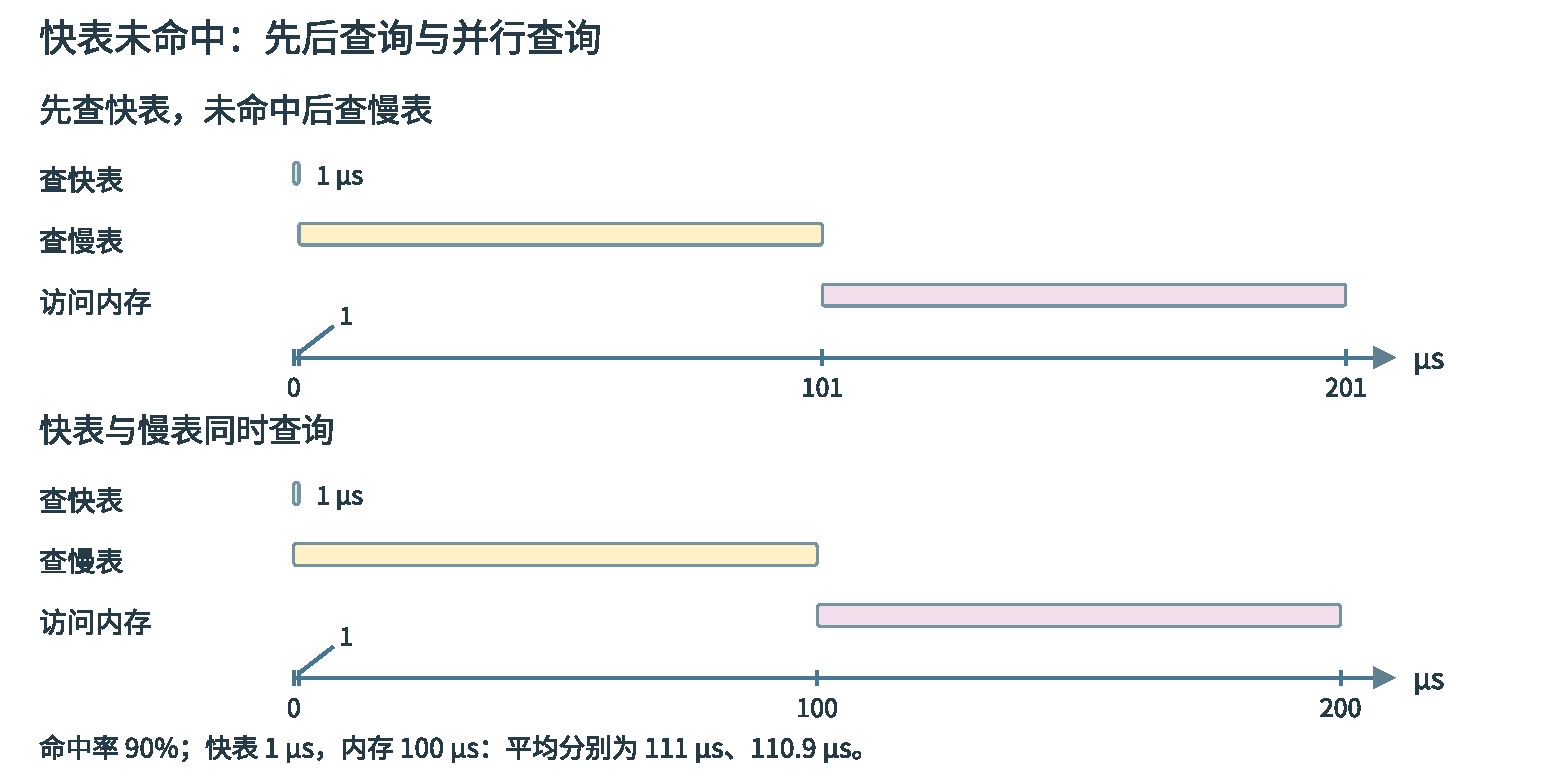
\includegraphics[width=\linewidth,height=125mm,keepaspectratio]{figures/OS03_tlb_time.pdf}
\captionof{figure}{快表未命中时串行与并行查询的时序比较}\label{os03-tlb-time}
\end{minipage}\par\medskip

\end{wideblock}

\section{分段和段页式：先检查段内地址}\label{OS03-5-6}

\textbf{分段}按程序的逻辑单位划分地址空间，例如代码段、数据段、栈段，每段长度可不同。逻辑地址用``段号、段内偏移''表示；段表记录段基址、段长和保护等。段号要落在段表范围内，偏移要小于段长，权限要允许本次操作，然后才计算基址与偏移之和。

\textbf{课件分段例。} 段2的基址为40 KiB，段内偏移为1024 B。先检查段2存在、权限满足且1024小于段长；这些条件成立时，物理地址为 \(40\times1024+1024=41984\)。若偏移越界，不能直接用基址相加所得值作为有效访问地址。

\begin{wideblock}

\par\medskip\noindent\begin{minipage}{\linewidth}
\centering
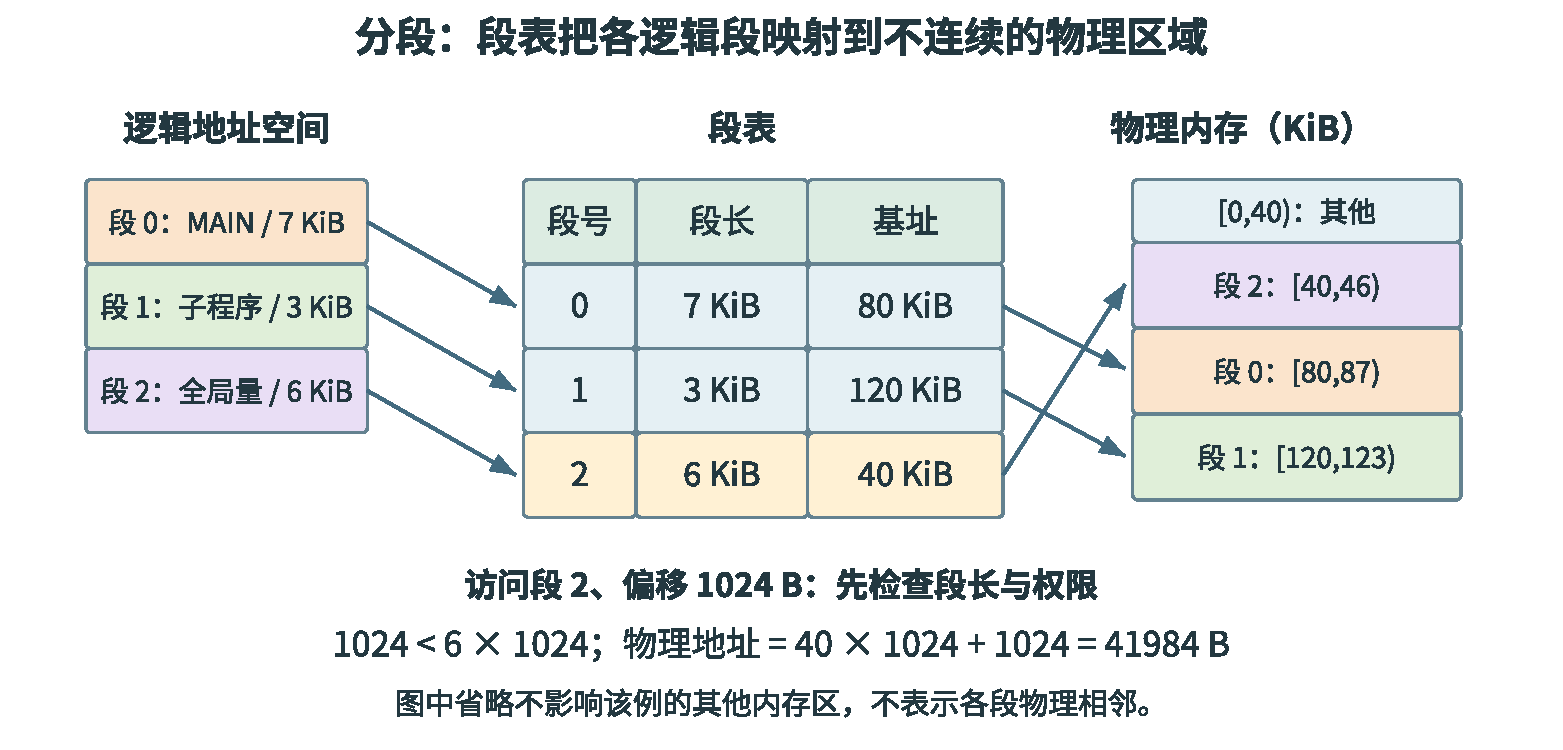
\includegraphics[width=\linewidth,height=125mm,keepaspectratio]{figures/OS03_segment_course.pdf}
\captionof{figure}{三个逻辑段经段表映射至非相邻物理内存区间}\label{os03-segment-course}
\end{minipage}\par\medskip

\end{wideblock}

\textbf{段页式}先按逻辑意义分段，再把各段分页；段表指向本段页表，页表再映射页框。它用段组织逻辑单位，用页框安排物理存储，不是``先把物理内存分段，再统一分页''。

转换时先检查段号和段级权限，再按段表给出的页表长度检查段内页号，合法后才查该段页表。题设若另外给出以字节为单位的段长，还须检查完整段内偏移是否越界；末页存在于内存，不会自动取消这个段长限制。

\begin{wideblock}

\par\medskip\noindent\begin{minipage}{\linewidth}\fontsize{9.3}{12}\selectfont\begin{tabularx}{\linewidth}{@{}YYYY@{}}
\toprule\noalign{}
\begin{minipage}[b]{\linewidth}\raggedright
比较维度
\end{minipage} & \begin{minipage}[b]{\linewidth}\raggedright
基本分页
\end{minipage} & \begin{minipage}[b]{\linewidth}\raggedright
基本分段
\end{minipage} & \begin{minipage}[b]{\linewidth}\raggedright
段页式
\end{minipage} \\
\midrule\noalign{}


划分依据和大小 & 系统规定的定长页，与程序逻辑模块无必然对应 & 代码、数据等逻辑单位，段长可变 & 先按逻辑分段，各段再分成定长页 \\
地址怎样解释 & 线性地址拆为页号、页内偏移 & 段号、段内偏移 & 段号、段内页号、页内偏移；后两项来自段内地址 \\
对程序的可见性 & 分页通常对程序透明 & 显式区分各逻辑段 & 段可见，段内分页通常透明 \\
物理连续性与碎片 & 页内连续，页间可离散；末页可能有内部碎片 & 每段连续，段间可离散；可能有外部碎片 & 每页内连续，同一段可跨离散页框；各段末页可能有内部碎片 \\
共享与保护 & 通过页映射和逐页权限实现 & 以完整逻辑段为单位较直观 & 段级逻辑组织与页级物理映射共同起作用 \\
基本地址转换路径 & 页表\ensuremath{\to}目标单元 & 段表\ensuremath{\to}目标单元 & 段表\ensuremath{\to}本段页表\ensuremath{\to}目标单元 \\
\bottomrule\end{tabularx}
\end{minipage}\par\medskip

\end{wideblock}

最后一行若按\textbf{单级页表、各表均在主存、没有 TLB 或其他缓存命中，也不发生缺页、越界或权限异常}计算，分别需要2、2、3次主存访问。改为多级页表或引入 TLB 后，应按实际路径重新计数。

【配套例题】 某进程段表如下，访问段号 2、段内地址 400 的逻辑地址，结果是（　）。

\begin{wideblock}

\par\medskip\noindent\begin{minipage}{\linewidth}\fontsize{9.3}{12}\selectfont\begin{tabularx}{\linewidth}{@{}YYYY@{}}
\toprule\noalign{}
段号 & 段长 & 内存起始地址 & 权限 \\
\midrule\noalign{}


0 & 100 & 6000 & 只读 \\
1 & 200 & --- & 读写 \\
2 & 300 & 4000 & 读写 \\
\bottomrule\end{tabularx}
\end{minipage}\par\medskip

\end{wideblock}

\begin{wideblock}

\par\medskip\noindent\begin{minipage}{\linewidth}\fontsize{9.3}{12}\selectfont\begin{tabularx}{\linewidth}{@{}YY@{}}
\toprule\noalign{}
段号 & 状态 \\
\midrule\noalign{}


0 & 在内存 \\
1 & 不在内存 \\
2 & 在内存 \\
\bottomrule\end{tabularx}
\end{minipage}\par\medskip

\end{wideblock}

A. 段缺失异常　　B. 内存地址 4400\\
C. 越权异常　　D. 越界异常

段 2 虽驻留且可读写，但偏移 \(400\ge300\)，已经越界，答案为 \textbf{D}。必须先检查长度，不能直接得到 4400。这里的数字是题设地址单位，不必自行加上 KB。

\subsection{段内分页的空间与地址维度}\label{OS03-segment-pages}

课件程序的三个逻辑段分别为MAIN 7 KiB、X 3 KiB、D 6 KiB，页大小4 KiB，则分别需要2、1、2页，共5页、20 KiB，最后一页未用空间分别为1、1、2 KiB，共4 KiB。每段在逻辑上完整，物理上则可分散到不同页框。

\par\medskip\noindent\begin{minipage}{\linewidth}
\centering
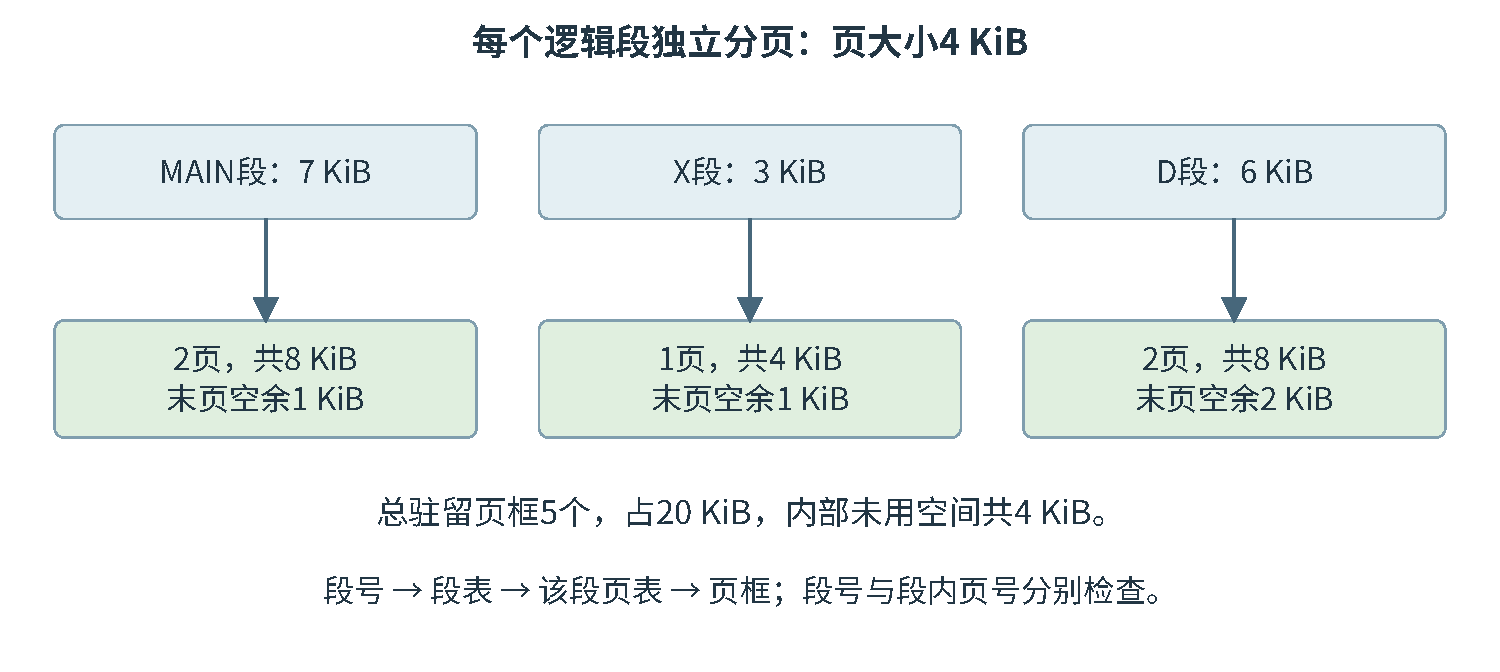
\includegraphics[width=\linewidth,height=125mm,keepaspectratio]{figures/OS_segment_pages.pdf}
\captionof{figure}{每个逻辑段分别分页，段表定位该段页表，页表定位物理页框}\label{os-fig-segment-pages}
\end{minipage}\par\medskip

若地址字段依次为段号16位、段内页号4位、页内偏移12位，最大段数为\(2^{16}\)，每段最多16页，每页4 KiB。程序通常给出``段号、段内地址''两个独立逻辑坐标，硬件再把段内地址拆成页号和偏移，所以该教材模型仍把段页式地址视为二维；地址编码出现三个字段不自动等于三个独立逻辑维度。

基本转换中先读段表取得该段页表位置和长度，再读页表取得页框，最后读目标。段号与页号都要分别检查，不能因高层查到一个表项就跳过下层越界判断。

\section{请求分页：合法但不驻留时会发生什么}\label{OS03-5-7}

\textbf{局部性}是程序在一段时期内倾向反复访问某些对象或其相邻位置。时间局部性来自循环与重用，空间局部性来自顺序指令、数组邻近元素等。虚拟内存利用这种特征，只保留当前所需部分，并在需要时调入其他部分，不要求整个进程同时装入。

请求分页的页表项需要区分页面是否驻留，并记录调页所需位置与状态。存在位表示是否在内存；访问位帮助估计近期使用；修改位表示装入后是否被写过，关系到淘汰时是否必须回写。\textbf{修改位不是写权限位}：允许写但尚未写的页可以是可写且 M=0；只读保护检查则发生在实际写入前。

\begin{wideblock}

\par\medskip\noindent\begin{minipage}{\linewidth}\fontsize{9.3}{12}\selectfont\begin{tabularx}{\linewidth}{@{}YYY@{}}
\toprule\noalign{}
\begin{minipage}[b]{\linewidth}\raggedright
比较维度
\end{minipage} & \begin{minipage}[b]{\linewidth}\raggedright
基本分页
\end{minipage} & \begin{minipage}[b]{\linewidth}\raggedright
请求分页
\end{minipage} \\
\midrule\noalign{}


执行前的驻留要求 & 按基本模型，待运行程序所需页面先装入内存 & 可先装入一部分，合法页面允许暂不驻留 \\
映射记录承担什么 & 给出页到页框的映射与相应保护信息 & 还需驻留状态、调页位置及置换所需的访问、修改等信息 \\
TLB 未命中以后 & 查主存页表取得已有映射 & 先查页表；驻留则继续，不驻留才进入缺页分支 \\
内存不足时怎样继续 & 不能只靠基本分页的地址变换解决 & 可能置换、必要时回写，再调入并更新映射 \\
本次指令怎样结束 & 正常转换后访问目标单元 & 缺页处理完成后重试原访存；异常处理开销不能漏计 \\
\bottomrule\end{tabularx}
\end{minipage}\par\medskip

\end{wideblock}

TLB 是地址转换缓存，基本分页和请求分页都可以使用它；是否有 TLB 与是否允许缺页是两个维度。

一次访存的处理应按执行顺序展开：检查地址合法性，查询 TLB/页表并检查存在状态与访问权限；合法但不驻留则引发缺页异常，内核定位后备内容，取得空闲页框或选择牺牲页；牺牲页若为脏页且需要保留则回写，调入所需页，更新页表和 TLB，重新执行被中断的访存。访问非法地址应按错误处理，不能一概``给它调一页''。

\par\medskip\noindent\begin{minipage}{\linewidth}
\centering
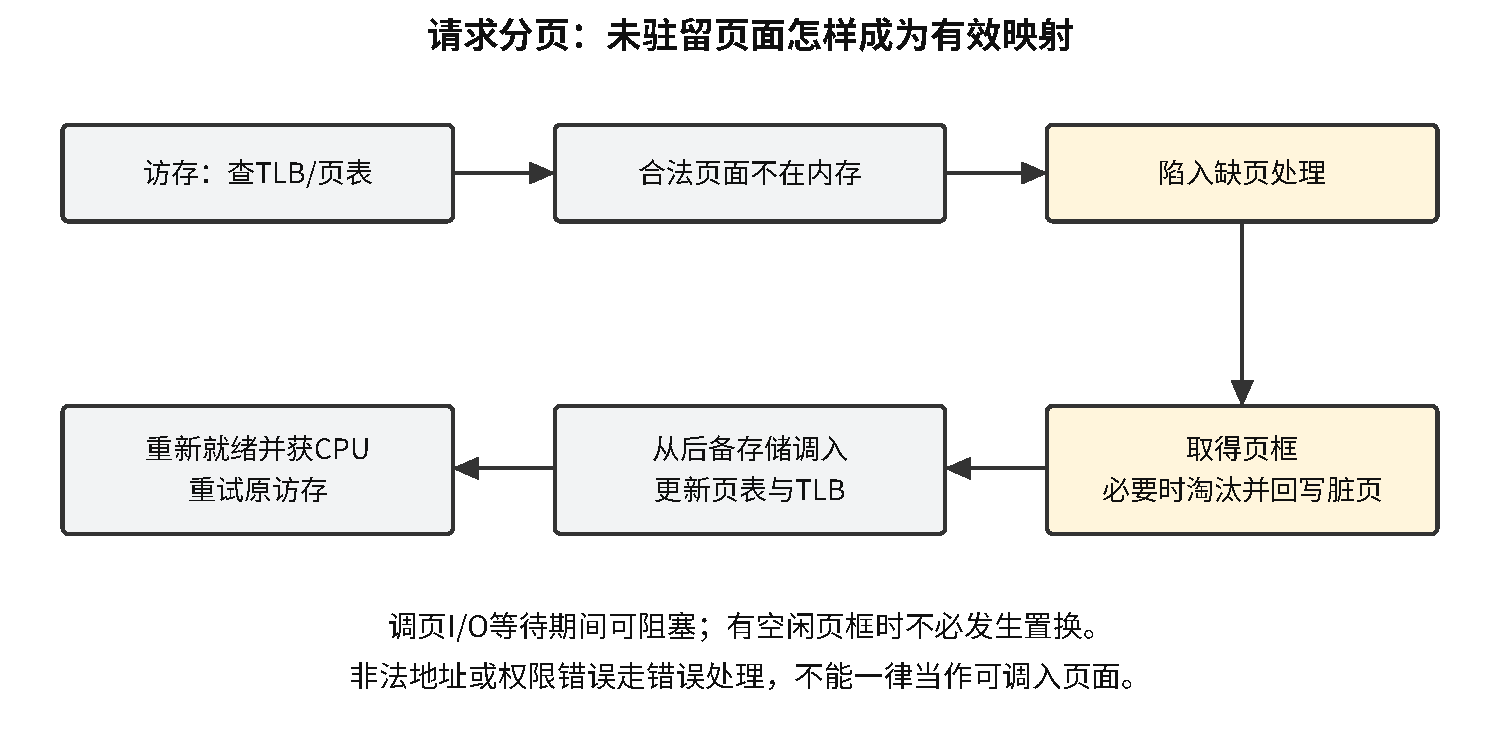
\includegraphics[width=\linewidth,height=125mm,keepaspectratio]{figures/OS_page_fault.pdf}
\captionof{figure}{缺页处理会阻塞等待 I/O；页面就绪以后还要重试原访存}\label{os-fig-fault}
\end{minipage}\par\medskip

\subsection{课件示例：空闲页框与脏页置换}\label{OS03-course-fault-states}

假设请求页0、页内偏移1024。页表中页0当前不驻留，其后备地址为x；页1驻留页框b，页2驻留页框c且已修改。访问字段10和6是该课件用于置换参考的记录值，不是单个访问位。

\textbf{处理前：}

\begin{wideblock}\par\medskip\noindent\begin{minipage}{\linewidth}\fontsize{9.3}{12}\selectfont\begin{tabularx}{\linewidth}{@{}YYYYYY@{}}
\toprule\noalign{}
页号 & 内存页框 & 状态位 & 访问字段 & 修改位 & 外存地址 \\
\midrule\noalign{}


0 & --- & 0 & 0 & 0 & x \\
1 & b & 1 & 10 & 0 & y \\
2 & c & 1 & 6 & 1 & z \\
\bottomrule\end{tabularx}
\end{minipage}\par\medskip\end{wideblock}

\begin{wideblock}

\par\medskip\noindent\begin{minipage}{\linewidth}
\centering
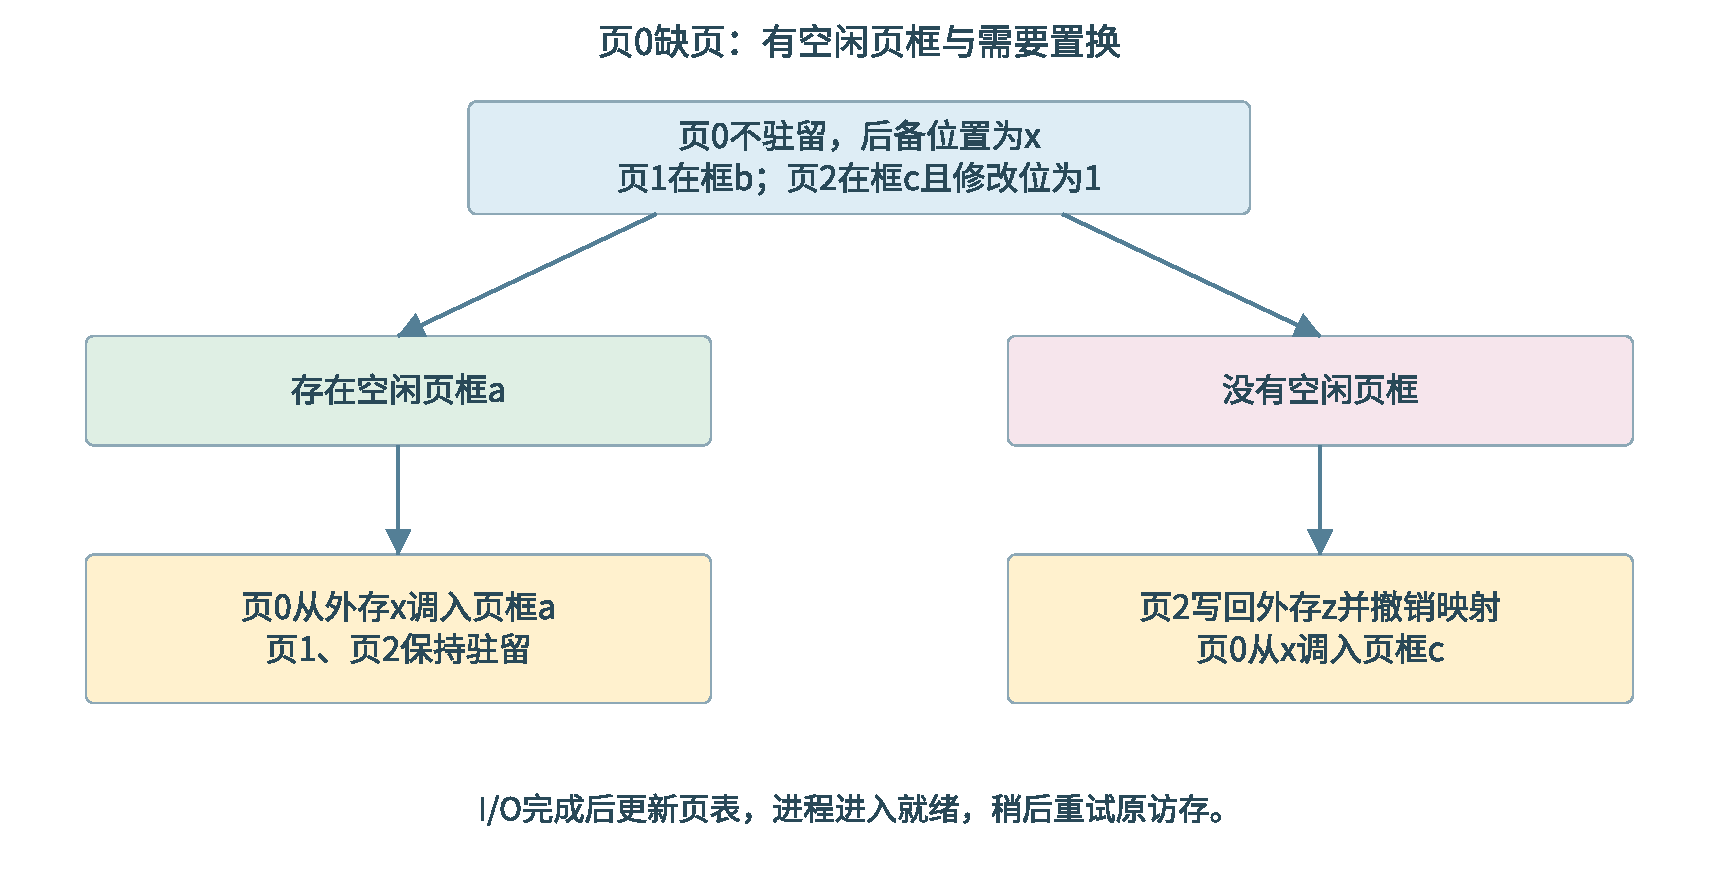
\includegraphics[width=\linewidth,height=125mm,keepaspectratio]{figures/OS03_fault_states_course.pdf}
\captionof{figure}{页0缺页后，有空闲页框和需要回写置换的两条处理路径}\label{os-fig-fault-states-course}
\end{minipage}\par\medskip

\end{wideblock}

\textbf{有空闲页框a：} 将页0从外存x调入a，页1、页2维持原映射，调入后页表为：

\begin{wideblock}\par\medskip\noindent\begin{minipage}{\linewidth}\fontsize{9.3}{12}\selectfont\begin{tabularx}{\linewidth}{@{}YYYYYY@{}}
\toprule\noalign{}
页号 & 内存页框 & 状态位 & 访问字段 & 修改位 & 外存地址 \\
\midrule\noalign{}


0 & a & 1 & 0 & 0 & x \\
1 & b & 1 & 10 & 0 & y \\
2 & c & 1 & 6 & 1 & z \\
\bottomrule\end{tabularx}
\end{minipage}\par\medskip\end{wideblock}

\textbf{没有空闲页框：} 假设置换算法选中页2，因修改位为1，先将页2写回外存z，再将页0从x调入框c并更新映射。页2已不驻留，状态位变为0。更新后、重试原访问前的课件页表为：

\begin{wideblock}\par\medskip\noindent\begin{minipage}{\linewidth}\fontsize{9.3}{12}\selectfont\begin{tabularx}{\linewidth}{@{}YYYYYY@{}}
\toprule\noalign{}
页号 & 内存页框 & 状态位 & 访问字段 & 修改位 & 外存地址 \\
\midrule\noalign{}


0 & c & 1 & 0 & 0 & x \\
1 & b & 1 & 10 & 0 & y \\
2 & --- & 0 & 0 & 0 & z \\
\bottomrule\end{tabularx}
\end{minipage}\par\medskip\end{wideblock}

表中的访问字段按课件所展示的处理时刻记录，进程之后重试访问时，系统可按采用的访问统计规则更新它；页2的修改内容必须在复用c前完成相应回写。

缺页不一定发生置换：有空闲页框就可直接装入。此外，一次复杂指令可能访问多个页面，执行期间可能产生不止一次缺页，系统必须保存足够的重启状态；最少页框数还受指令寻址方式等约束。页面置换算法不能改变``一条指令所需页面无论如何无法同时提供''这一基本执行条件。

\section{页框分配与置换范围}\label{OS03-5-8}

\textbf{驻留集}是进程当前在内存的页面集合。固定分配是指给每个进程固定数量的页框；可变分配允许按运行状况调整。\textbf{局部置换}只在本进程驻留集中选牺牲页；\textbf{全局置换}可从其他进程等更大集合中选择，会改变各进程实际占有的页框量。

因此经典组合中，固定分配通常配局部置换；可变分配可以局部或全局置换。把固定分配与全局置换直接组合，会使被换出进程的页框量改变，违背这里``固定''的约定。常用的分配方法有平均分配、按进程大小分配和按优先级分配等，但还须满足体系结构要求的最少页框数。

请求调页在真正缺页时装入，能减少无用装入；预调页根据局部性提前带入可能需要的内容，可以减少后续等待，也可能调入没用的页。回写策略、清洁页缓冲和空闲页队列影响缺页处理代价，不能只看替换算法的名称。

\subsection{调入来源、锁定页与虚拟内存特征}\label{OS03-backing}

\textbf{课件容量例。} 32位字节地址的寻址上限为 \(2^{32}\) B，即4 GiB。若抽象模型假设512 MiB物理内存和2 GiB后备外存均可用于该进程，则课件模型的可支持量为 \(\min(4\text{ GiB},512\text{ MiB}+2\text{ GiB})=2.5\text{ GiB}\)。这是在给定后备容量和使用条件下的示例：实际系统还受到地址保留、共享映射、后备策略和资源限制，不能把物理内存与整块磁盘容量相加当成无条件结论。

虚拟内存的\textbf{多次性}指运行信息可以分多次装入，\textbf{对换性}指运行期间允许将暂不用内容换出、需要时再换入，\textbf{虚拟性}指向程序提供的逻辑使用空间可以超过当前可分配物理内存。虚拟容量首先受地址表示范围约束，也受系统映射与后备能力限制；物理内存和磁盘的简单相加不能替代这些约束。

\textbf{课件容量例。} 按字节编址，逻辑地址为32位，内存为512 MiB、外存为2 GiB，地址表示范围为 \(2^{32}\) B，即4 GiB。课件采用理想化估算：以给定内存、外存容量之和作为可提供空间，再取其与地址范围的较小值，得到 \(\min(4,\,0.5+2)=2.5\) GiB。实际系统还受可用后备空间、保留区域和映射策略约束，不能默认整块外存都可用于该进程。

调页必须知道页面的后备位置。未修改且有有效文件副本的页面，淘汰时可以丢弃内存副本，下次从文件重读；需要保留的脏页则须写到规定的文件或对换区域。匿名页、私有映射与共享文件映射的后备关系不同，写回对象要按模型确定。

部分关键内核页或设备正在直接使用的页会被锁定，不能作为一般置换候选。

页框分配可采用平均、按大小比例或按优先级等方法，最少页框数还要满足一条指令及其寻址过程的需求。可变分配的缺页率控制依据一段运行观察调整资源，某一次缺页本身并不证明进程长期驻留集不足。

\subsection{三种调入与调出组织}\label{OS03-backing-course-models}

下面三种组织是讨论页面后备位置的典型模型。\textbf{对换区充足}时，在进程运行之前，可将有关文件内容复制到对换区，运行中的页面调入和调出均在内存与对换区之间进行。这样可在课件给出的对换区连续分配模型下减少相应磁盘访问开销；具体性能仍取决于实际存储设备和实现。

\textbf{对换区不足}时，可将不会修改的数据保留在文件区，每次需要时从文件区调入；这类页面未被修改，换出时可以丢弃内存副本。需要保留修改的数据在换出时写入对换区，再次需要时从对换区调入。

\textbf{UNIX式模型}中，尚未使用的页面第一次可从文件区调入；页面被换出并保存到对换区后，再次使用时从对换区调入。是否确实需要回写仍由页面状态与具体实现决定，图中表示该模型的调入来源关系。

\begin{wideblock}

\par\medskip\noindent\begin{minipage}{\linewidth}
\centering
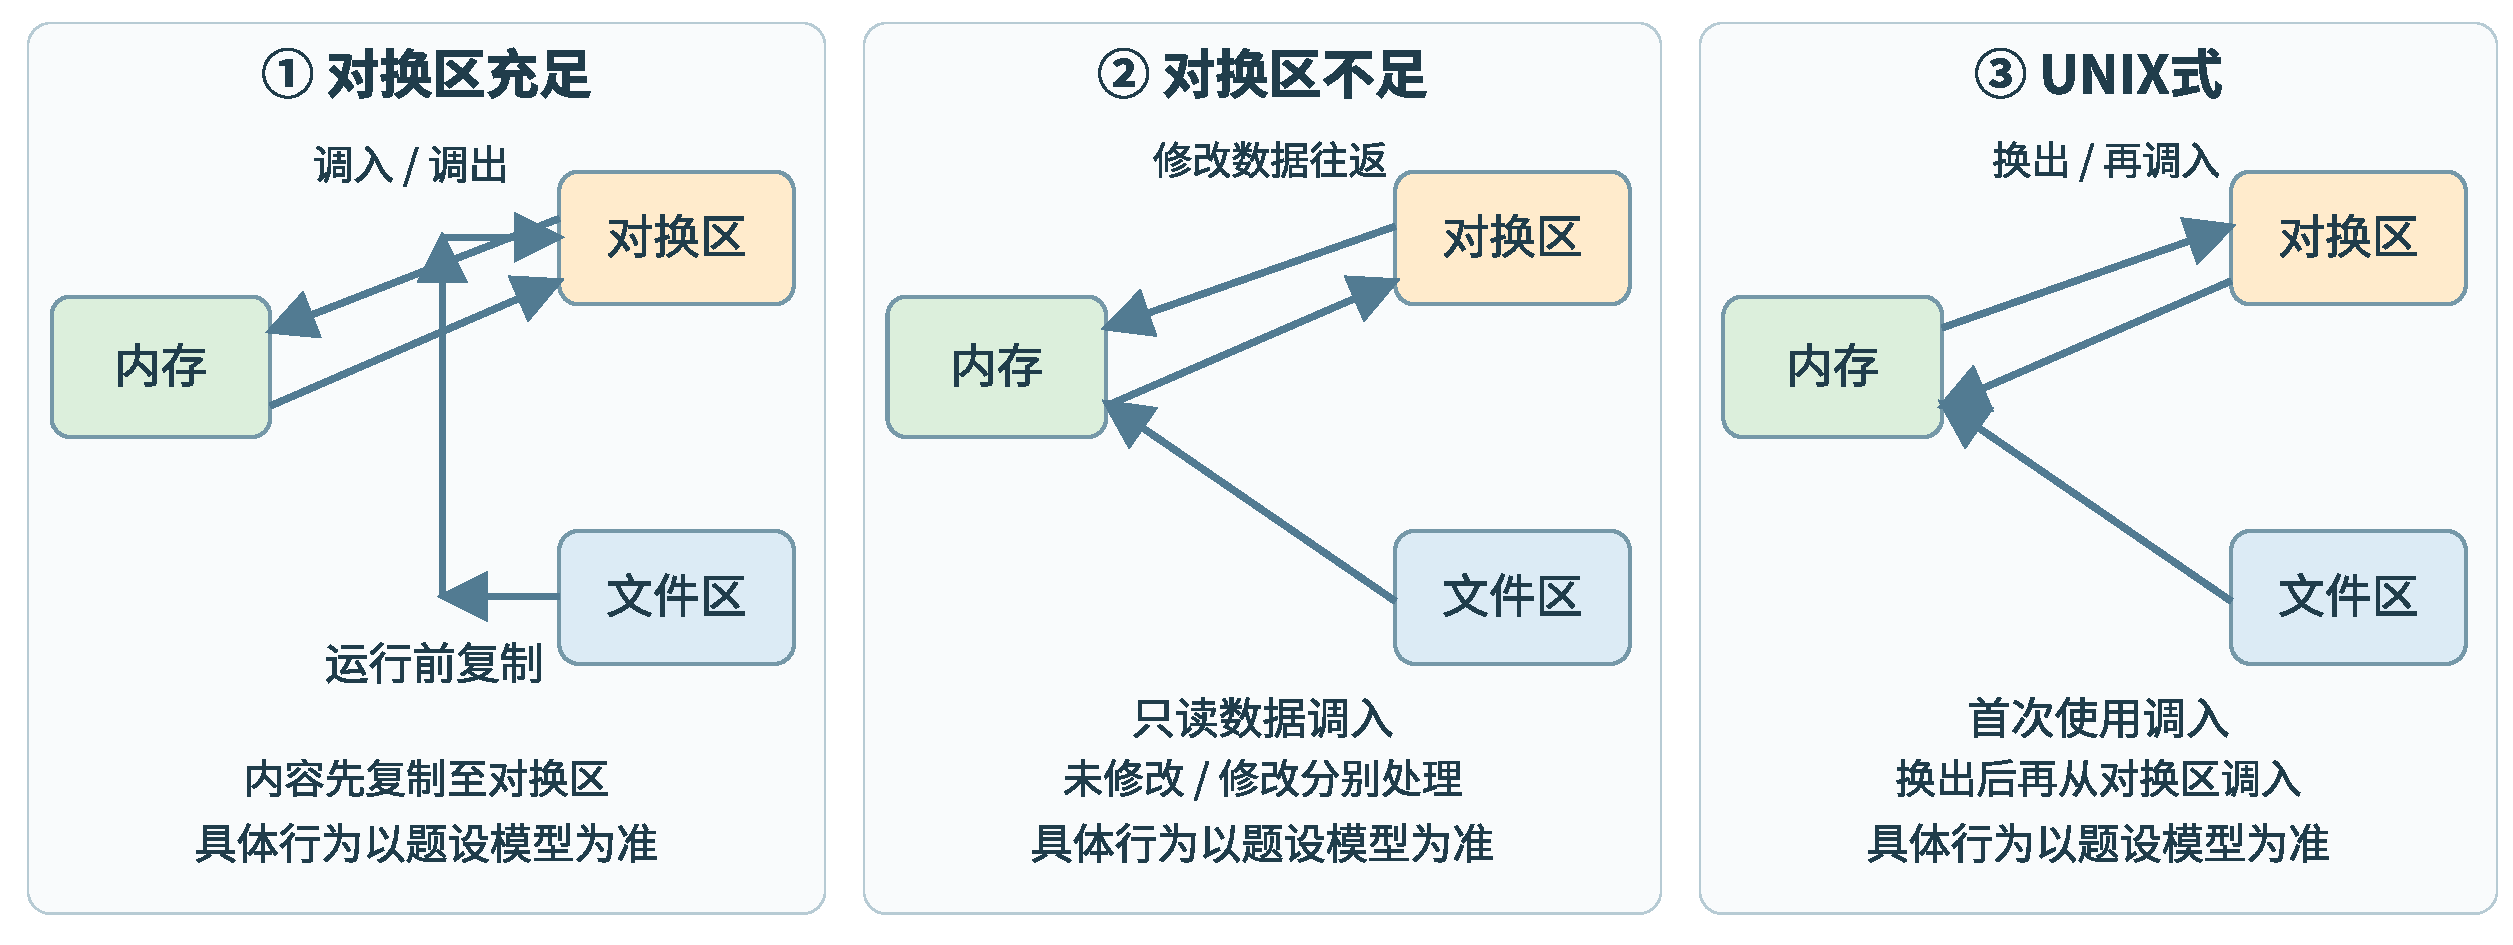
\includegraphics[width=\linewidth,height=125mm,keepaspectratio]{figures/OS03_page_backing_models_course.pdf}
\captionof{figure}{对换区充足、对换区不足及UNIX式模型中，内存、文件区与对换区之间的调入和调出方向}\label{os03-backing-models}
\end{minipage}\par\medskip

\end{wideblock}

\section{页面置换：必须跟踪实际状态}\label{OS03-5-9}

\textbf{OPT}淘汰未来最长时间不再访问的页，未来不再访问者优先；它需要未来信息，主要用作比较基准。\textbf{FIFO}淘汰最早装入者，命中通常不改变装入顺序。\textbf{LRU}淘汰最近最久未使用者，每次命中也要更新最近使用关系。若只在缺页时更新 LRU 次序，实现出来就接近 FIFO。

\subsection{王道课件中的四组置换轨迹}\label{OS03-course-replacement-traces}

下表按固定物理页框编号展示每次访问后的状态；``---''表示尚为空，``命''表示命中，``装''表示缺页后使用空框，``换x''表示缺页并淘汰页x。每组从空页框开始；缺页次数包含初次装入，置换次数只统计淘汰原页。

\textbf{OPT，3个页框。} 引用串：7、0、1、2、0、3、0、4、2、3、0、3、2、1、2、0、1、7、0、1。共缺页9次，其中置换6次。

\begin{wideblock}\par\medskip\noindent\begin{minipage}{\linewidth}\fontsize{9.3}{12}\selectfont\begin{tabularx}{\linewidth}{@{}YYYYYYY@{}}
\toprule\noalign{}
步骤 & 1 & 2 & 3 & 4 & 5 & 6 \\
\midrule\noalign{}


访问页 & 7 & 0 & 1 & 2 & 0 & 3 \\
页框1 & 7 & 7 & 7 & 2 & 2 & 2 \\
页框2 & --- & 0 & 0 & 0 & 0 & 0 \\
页框3 & --- & --- & 1 & 1 & 1 & 3 \\
结果 & 装 & 装 & 装 & 换7 & 命 & 换1 \\
\bottomrule\end{tabularx}
\end{minipage}\par\medskip\end{wideblock}

\begin{wideblock}\par\medskip\noindent\begin{minipage}{\linewidth}\fontsize{9.3}{12}\selectfont\begin{tabularx}{\linewidth}{@{}YYYYYYY@{}}
\toprule\noalign{}
步骤 & 7 & 8 & 9 & 10 & 11 & 12 \\
\midrule\noalign{}


访问页 & 0 & 4 & 2 & 3 & 0 & 3 \\
页框1 & 2 & 2 & 2 & 2 & 2 & 2 \\
页框2 & 0 & 4 & 4 & 4 & 0 & 0 \\
页框3 & 3 & 3 & 3 & 3 & 3 & 3 \\
结果 & 命 & 换0 & 命 & 命 & 换4 & 命 \\
\bottomrule\end{tabularx}
\end{minipage}\par\medskip\end{wideblock}

\begin{wideblock}\par\medskip\noindent\begin{minipage}{\linewidth}\fontsize{9.3}{12}\selectfont\begin{tabularx}{\linewidth}{@{}YYYYYYY@{}}
\toprule\noalign{}
步骤 & 13 & 14 & 15 & 16 & 17 & 18 \\
\midrule\noalign{}


访问页 & 2 & 1 & 2 & 0 & 1 & 7 \\
页框1 & 2 & 2 & 2 & 2 & 2 & 7 \\
页框2 & 0 & 0 & 0 & 0 & 0 & 0 \\
页框3 & 3 & 1 & 1 & 1 & 1 & 1 \\
结果 & 命 & 换3 & 命 & 命 & 命 & 换2 \\
\bottomrule\end{tabularx}
\end{minipage}\par\medskip\end{wideblock}

\par\medskip\noindent\begin{minipage}{\linewidth}\fontsize{9.3}{12}\selectfont\begin{tabularx}{\linewidth}{@{}YYY@{}}
\toprule\noalign{}
步骤 & 19 & 20 \\
\midrule\noalign{}


访问页 & 0 & 1 \\
页框1 & 7 & 7 \\
页框2 & 0 & 0 \\
页框3 & 1 & 1 \\
结果 & 命 & 命 \\
\bottomrule\end{tabularx}
\end{minipage}\par\medskip

例如第4步访问2时，在现有7、0、1中，7下一次出现在第18步，晚于0和1，故淘汰7；未来不再访问的页可优先淘汰。

\textbf{FIFO，3个页框。} 引用串：3、2、1、0、3、2、4、3、2、1、0、4。共缺页9次，其中置换6次。

\begin{wideblock}\par\medskip\noindent\begin{minipage}{\linewidth}\fontsize{9.3}{12}\selectfont\begin{tabularx}{\linewidth}{@{}YYYYYYY@{}}
\toprule\noalign{}
步骤 & 1 & 2 & 3 & 4 & 5 & 6 \\
\midrule\noalign{}


访问页 & 3 & 2 & 1 & 0 & 3 & 2 \\
页框1 & 3 & 3 & 3 & 0 & 0 & 0 \\
页框2 & --- & 2 & 2 & 2 & 3 & 3 \\
页框3 & --- & --- & 1 & 1 & 1 & 2 \\
结果 & 装 & 装 & 装 & 换3 & 换2 & 换1 \\
\bottomrule\end{tabularx}
\end{minipage}\par\medskip\end{wideblock}

\begin{wideblock}\par\medskip\noindent\begin{minipage}{\linewidth}\fontsize{9.3}{12}\selectfont\begin{tabularx}{\linewidth}{@{}YYYYYYY@{}}
\toprule\noalign{}
步骤 & 7 & 8 & 9 & 10 & 11 & 12 \\
\midrule\noalign{}


访问页 & 4 & 3 & 2 & 1 & 0 & 4 \\
页框1 & 4 & 4 & 4 & 4 & 4 & 4 \\
页框2 & 3 & 3 & 3 & 1 & 1 & 1 \\
页框3 & 2 & 2 & 2 & 2 & 0 & 0 \\
结果 & 换0 & 命 & 命 & 换3 & 换2 & 命 \\
\bottomrule\end{tabularx}
\end{minipage}\par\medskip\end{wideblock}

\textbf{FIFO，4个页框。} 引用串：3、2、1、0、3、2、4、3、2、1、0、4。共缺页10次，其中置换6次。

\begin{wideblock}\par\medskip\noindent\begin{minipage}{\linewidth}\fontsize{9.3}{12}\selectfont\begin{tabularx}{\linewidth}{@{}YYYYYYY@{}}
\toprule\noalign{}
步骤 & 1 & 2 & 3 & 4 & 5 & 6 \\
\midrule\noalign{}


访问页 & 3 & 2 & 1 & 0 & 3 & 2 \\
页框1 & 3 & 3 & 3 & 3 & 3 & 3 \\
页框2 & --- & 2 & 2 & 2 & 2 & 2 \\
页框3 & --- & --- & 1 & 1 & 1 & 1 \\
页框4 & --- & --- & --- & 0 & 0 & 0 \\
结果 & 装 & 装 & 装 & 装 & 命 & 命 \\
\bottomrule\end{tabularx}
\end{minipage}\par\medskip\end{wideblock}

\begin{wideblock}\par\medskip\noindent\begin{minipage}{\linewidth}\fontsize{9.3}{12}\selectfont\begin{tabularx}{\linewidth}{@{}YYYYYYY@{}}
\toprule\noalign{}
步骤 & 7 & 8 & 9 & 10 & 11 & 12 \\
\midrule\noalign{}


访问页 & 4 & 3 & 2 & 1 & 0 & 4 \\
页框1 & 4 & 4 & 4 & 4 & 0 & 0 \\
页框2 & 2 & 3 & 3 & 3 & 3 & 4 \\
页框3 & 1 & 1 & 2 & 2 & 2 & 2 \\
页框4 & 0 & 0 & 0 & 1 & 1 & 1 \\
结果 & 换3 & 换2 & 换1 & 换0 & 换4 & 换3 \\
\bottomrule\end{tabularx}
\end{minipage}\par\medskip\end{wideblock}

同一引用串下，FIFO从三个页框增加到四个页框，缺页从9次增加到10次，出现Belady异常；命中不改变FIFO的装入顺序。

\textbf{LRU，4个页框。} 引用串：1、8、1、7、8、2、7、2、1、8、3、8、2、1、3、1、7、1、3、7。共缺页6次，其中置换2次。

\begin{wideblock}\par\medskip\noindent\begin{minipage}{\linewidth}\fontsize{9.3}{12}\selectfont\begin{tabularx}{\linewidth}{@{}YYYYYYY@{}}
\toprule\noalign{}
步骤 & 1 & 2 & 3 & 4 & 5 & 6 \\
\midrule\noalign{}


访问页 & 1 & 8 & 1 & 7 & 8 & 2 \\
页框1 & 1 & 1 & 1 & 1 & 1 & 1 \\
页框2 & --- & 8 & 8 & 8 & 8 & 8 \\
页框3 & --- & --- & --- & 7 & 7 & 7 \\
页框4 & --- & --- & --- & --- & --- & 2 \\
结果 & 装 & 装 & 命 & 装 & 命 & 装 \\
\bottomrule\end{tabularx}
\end{minipage}\par\medskip\end{wideblock}

\begin{wideblock}\par\medskip\noindent\begin{minipage}{\linewidth}\fontsize{9.3}{12}\selectfont\begin{tabularx}{\linewidth}{@{}YYYYYYY@{}}
\toprule\noalign{}
步骤 & 7 & 8 & 9 & 10 & 11 & 12 \\
\midrule\noalign{}


访问页 & 7 & 2 & 1 & 8 & 3 & 8 \\
页框1 & 1 & 1 & 1 & 1 & 1 & 1 \\
页框2 & 8 & 8 & 8 & 8 & 8 & 8 \\
页框3 & 7 & 7 & 7 & 7 & 3 & 3 \\
页框4 & 2 & 2 & 2 & 2 & 2 & 2 \\
结果 & 命 & 命 & 命 & 命 & 换7 & 命 \\
\bottomrule\end{tabularx}
\end{minipage}\par\medskip\end{wideblock}

\begin{wideblock}\par\medskip\noindent\begin{minipage}{\linewidth}\fontsize{9.3}{12}\selectfont\begin{tabularx}{\linewidth}{@{}YYYYYYY@{}}
\toprule\noalign{}
步骤 & 13 & 14 & 15 & 16 & 17 & 18 \\
\midrule\noalign{}


访问页 & 2 & 1 & 3 & 1 & 7 & 1 \\
页框1 & 1 & 1 & 1 & 1 & 1 & 1 \\
页框2 & 8 & 8 & 8 & 8 & 7 & 7 \\
页框3 & 3 & 3 & 3 & 3 & 3 & 3 \\
页框4 & 2 & 2 & 2 & 2 & 2 & 2 \\
结果 & 命 & 命 & 命 & 命 & 换8 & 命 \\
\bottomrule\end{tabularx}
\end{minipage}\par\medskip\end{wideblock}

\par\medskip\noindent\begin{minipage}{\linewidth}\fontsize{9.3}{12}\selectfont\begin{tabularx}{\linewidth}{@{}YYY@{}}
\toprule\noalign{}
步骤 & 19 & 20 \\
\midrule\noalign{}


访问页 & 3 & 7 \\
页框1 & 1 & 1 \\
页框2 & 7 & 7 \\
页框3 & 3 & 3 \\
页框4 & 2 & 2 \\
结果 & 命 & 命 \\
\bottomrule\end{tabularx}
\end{minipage}\par\medskip

第11步装入3时，7最近一次使用在第7步，早于其余驻留页，故淘汰7；第17步装入7时，8最久未用，故淘汰8。命中也必须更新最近使用时间。

\subsection{例 3-5　缺页次数与置换次数相差初装入次数}\label{OS03-ex5-5}

\begin{example}[配套例题]

【配套例题】 某系统采用 LRU 页置换和局部置换。为进程预分配 4 个页框，访问页号依次为 0、1、2、7、0、5、3、5、0、2、7、6。产生页面置换的总次数为（　）。

A. 3　　B. 4\\
C. 5　　D. 6

\end{example}

\textbf{解析。} 下表按“最久未用\ensuremath{\to}最近使用”记驻留页，因而每次命中也会移动相应页的位置；开始页框为空。

\begin{wideblock}

\par\medskip\noindent\begin{minipage}{\linewidth}\fontsize{9.3}{12}\selectfont\begin{tabularx}{\linewidth}{@{}YYY@{}}
\toprule\noalign{}
访问 & 访问后最近使用次序 & 结果 \\
\midrule\noalign{}


0 & 0 & 缺页，空框装入 \\
1 & 0、1 & 缺页，空框装入 \\
2 & 0、1、2 & 缺页，空框装入 \\
7 & 0、1、2、7 & 缺页，空框装入 \\
0 & 1、2、7、0 & 命中 \\
5 & 2、7、0、5 & 缺页，淘汰 1 \\
3 & 7、0、5、3 & 缺页，淘汰 2 \\
\bottomrule\end{tabularx}
\end{minipage}\par\medskip

\par\medskip\noindent\begin{minipage}{\linewidth}\fontsize{9.3}{12}\selectfont\begin{tabularx}{\linewidth}{@{}YYY@{}}
\toprule\noalign{}
访问 & 访问后最近使用次序 & 结果 \\
\midrule\noalign{}


5 & 7、0、3、5 & 命中 \\
0 & 7、3、5、0 & 命中 \\
2 & 3、5、0、2 & 缺页，淘汰 7 \\
7 & 5、0、2、7 & 缺页，淘汰 3 \\
6 & 0、2、7、6 & 缺页，淘汰 5 \\
\bottomrule\end{tabularx}
\end{minipage}\par\medskip

\end{wideblock}

共 9 次缺页，前 4 次利用空框，实际置换 5 次，答案为 \textbf{C}。题目问置换时，不要把所有缺页都记为替换。

\subsection{Clock 的访问位给页面第二次机会}\label{OS03-auto-3}

基本 Clock 把页框排成环，指针指向下一个候选。页面被访问时置 A=1；缺页需替换时，检查指针所指页，A=0 就选它，A=1 则清为 0 并前进，直到选中牺牲页。新装入并被本次访问的页设 A=1，指针前移。指针初始位置、装入后位置若题设另有规定，要按题设执行。

\textbf{课件Clock轨迹。} 五个空页框按1至5循环，初始指针指向页框1；引用串依次为1、3、4、2、5、6、3、4、7。装入页后访问位置1，指针前移；命中置访问位1但不移动置换指针。前五次装入后，页框为 \texttt{[\allowbreak{}1,\allowbreak{}3,\allowbreak{}4,\allowbreak{}2,\allowbreak{}5]\allowbreak{}}，访问位均为1，指针回到页框1。访问6缺页时，从页框1起依次将五个1清零，随后淘汰1并装入6，状态为 \texttt{[\allowbreak{}6,\allowbreak{}3,\allowbreak{}4,\allowbreak{}2,\allowbreak{}5]\allowbreak{}}、访问位 \texttt{[\allowbreak{}1,\allowbreak{}0,\allowbreak{}0,\allowbreak{}0,\allowbreak{}0]\allowbreak{}}，指针指向页框2。之后访问3、4命中，访问位变为 \texttt{[\allowbreak{}1,\allowbreak{}1,\allowbreak{}1,\allowbreak{}0,\allowbreak{}0]\allowbreak{}}；访问7缺页时，从页框2起依次清除3、4的访问位，在页框4遇到访问位0的2并淘汰，最终页框为 \texttt{[\allowbreak{}6,\allowbreak{}3,\allowbreak{}4,\allowbreak{}7,\allowbreak{}5]\allowbreak{}}、访问位 \texttt{[\allowbreak{}1,\allowbreak{}0,\allowbreak{}0,\allowbreak{}1,\allowbreak{}0]\allowbreak{}}，指针前移至页框5。五次初装加两次置换共7次缺页；如果题目规定了不同的指针推进规则，应按其规则重算。

\begin{wideblock}\par\medskip\noindent\begin{minipage}{\linewidth}\fontsize{9.3}{12}\selectfont\begin{tabularx}{\linewidth}{@{}YYYYY@{}}
\toprule\noalign{}
访问页 & 页框1至5 & 对应访问位 & 下一扫描页框 & 结果 \\
\midrule\noalign{}


1 & 1、---、---、---、--- & 1、---、---、---、--- & 2 & 装入空框 \\
3 & 1、3、---、---、--- & 1、1、---、---、--- & 3 & 装入空框 \\
4 & 1、3、4、---、--- & 1、1、1、---、--- & 4 & 装入空框 \\
2 & 1、3、4、2、--- & 1、1、1、1、--- & 5 & 装入空框 \\
5 & 1、3、4、2、5 & 1、1、1、1、1 & 1 & 装入空框 \\
6 & 6、3、4、2、5 & 1、0、0、0、0 & 2 & 置换1 \\
3 & 6、3、4、2、5 & 1、1、0、0、0 & 2 & 命中 \\
\bottomrule\end{tabularx}
\end{minipage}\par\medskip\end{wideblock}

\begin{wideblock}\par\medskip\noindent\begin{minipage}{\linewidth}\fontsize{9.3}{12}\selectfont\begin{tabularx}{\linewidth}{@{}YYYYY@{}}
\toprule\noalign{}
访问页 & 页框1至5 & 对应访问位 & 下一扫描页框 & 结果 \\
\midrule\noalign{}


4 & 6、3、4、2、5 & 1、1、1、0、0 & 2 & 命中 \\
7 & 6、3、4、7、5 & 1、0、0、1、0 & 5 & 置换2 \\
\bottomrule\end{tabularx}
\end{minipage}\par\medskip\end{wideblock}

\textbf{机制小例（原创）。} 四页框按环依次为 \(p,q,r,s\)，访问位为 1、0、1、0，指针从 p 开始。需淘汰时，先将 p 的 1 清 0，再选 q；r、s 本次未被扫描，原位不变。不能每次缺页都把所有访问位统一清零。这一小例只检查扫描中间状态，未替代真题的选页任务。

改进型 Clock 再考虑修改位。在本书采用的四类优先关系中，依次考虑 (A,M) 为 (0,0)、(0,1)、(1,0)、(1,1)：先选近期未访问且不需回写者，再考虑近期未访问的脏页，近期访问过者留待后续。具体多轮扫描会修改 A，必须按当时状态判断，不能把开始扫描前的分类当作固定次序。

按课件的四轮扫描规则，各轮均从本次置换开始时的指针位置出发，沿环的同一方向最多扫描一圈：

\begin{enumerate}
\def\labelenumi{\arabic{enumi}.}
\tightlist
\item
  寻找第一个 \((A,M)=(0,0)\) 的页，找到即选中；本轮不修改访问位。
\item
  若首轮失败，寻找第一个 \((0,1)\) 的页，找到即选中；对本轮经过但未选中的页，将其访问位清为 0。
\item
  若第二轮也失败，重新寻找第一个 \((0,0)\) 的页；本轮不修改访问位。
\item
  若第三轮失败，重新寻找第一个 \((0,1)\) 的页。经过完整的第二轮后，所有候选页的访问位都已清零，所以第三、第四轮中必能选出页面。
\end{enumerate}

扫描过程中页的类别会变化：第二轮被清零的 \((1,0)\) 可在第三轮变为 \((0,0)\)。因此，应逐轮执行并更新状态，不能只按最初的四类标签一次性排序。扫描只改变 A，M 不能因扫描而任意清零；脏内容完成相应回写后才能标记为干净。

图中的每个状态对按环次序排列，分别表示不同的候选集合；只给状态、未给扫描起点时，不能确定同类候选中最终选中的具体页框。状态1和状态3含\((0,0)\)，按第一轮规则选择扫描中第一个\((0,0)\)；状态2没有\((0,0)\)但有\((0,1)\)，首轮失败后第二轮可以选到扫描中第一个\((0,1)\)；状态4全部为\((0,1)\)，首轮失败，第二轮选中遇到的第一个页框。实际扫描时，应同步记录第二轮已经过页的访问位变化。

\begin{wideblock}

\par\medskip\noindent\begin{minipage}{\linewidth}
\centering
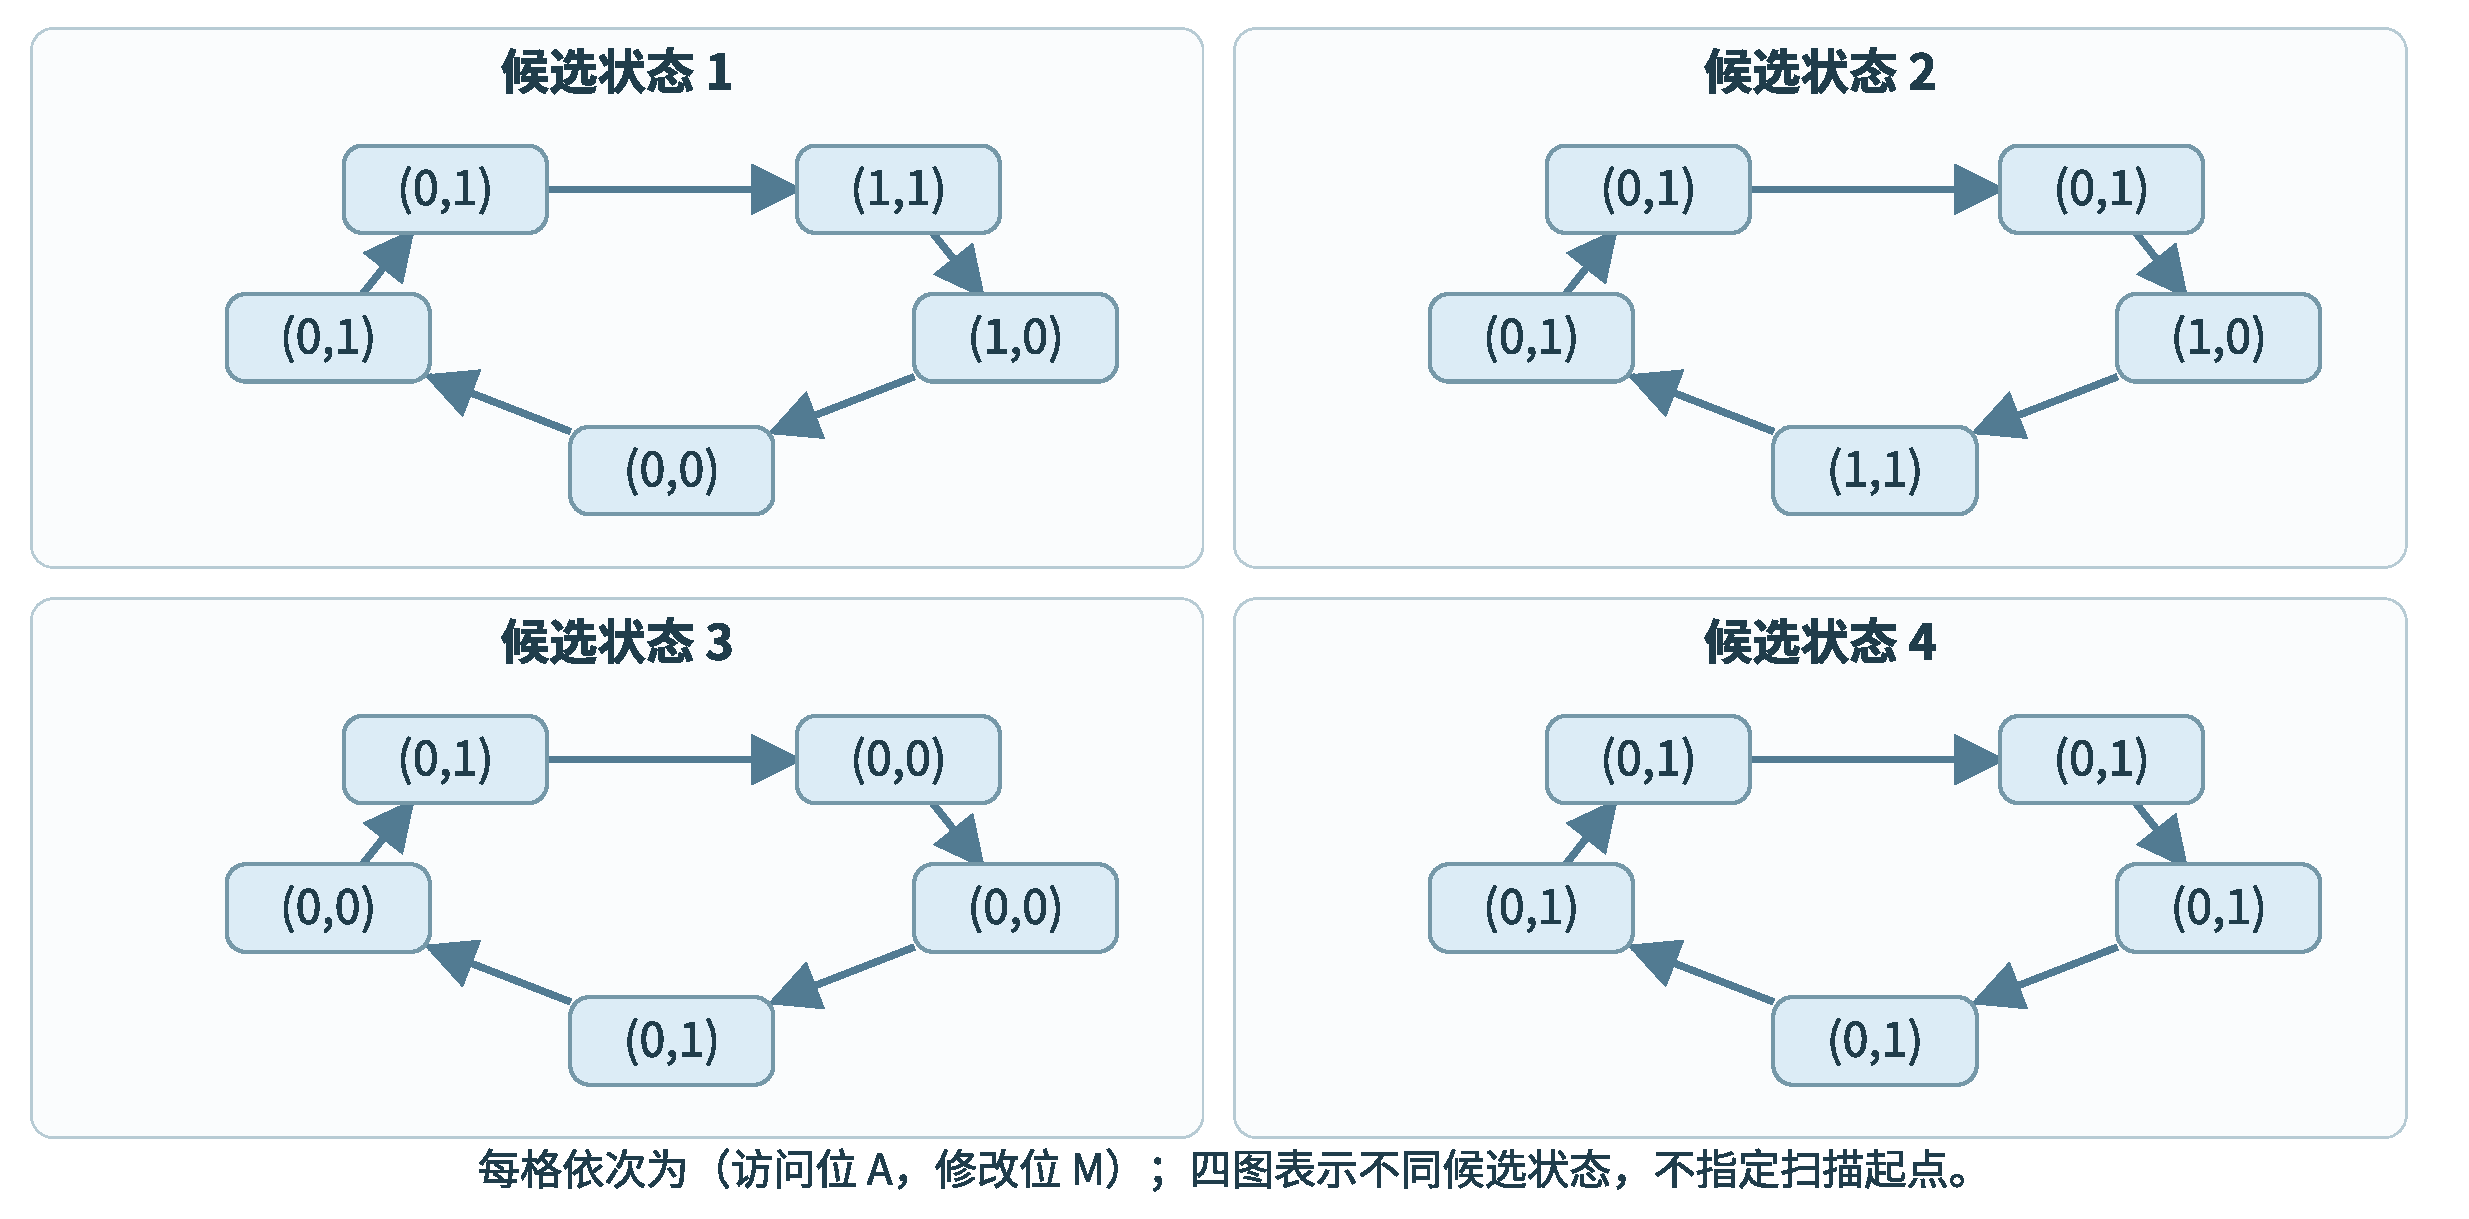
\includegraphics[width=\linewidth,height=125mm,keepaspectratio]{figures/OS03_improved_clock_states_course.pdf}
\captionof{figure}{改进型Clock四组环状候选状态；括号内依次是访问位与修改位}\label{os03-clock-states}
\end{minipage}\par\medskip

\end{wideblock}

\subsection{例 3-6　缺页后，旧页框字段不能直接沿用}\label{OS03-ex5-6}

\begin{example}[配套例题]

【配套例题】 某请求分页系统页大小为 4 KB，按字节编址。为进程 P 分配 2 个固定页框，采用改进型 Clock，页表部分内容如下。

\begin{wideblock}

\par\medskip\noindent\begin{minipage}{\linewidth}\fontsize{9.3}{12}\selectfont\begin{tabularx}{\linewidth}{@{}YYYY@{}}
\toprule\noalign{}
页号 & 页框号 & 存在位 & 访问位 \\
\midrule\noalign{}


2 & 20H & 0 & 0 \\
3 & 60H & 1 & 1 \\
4 & 80H & 1 & 1 \\
\bottomrule\end{tabularx}
\end{minipage}\par\medskip

\end{wideblock}

\begin{wideblock}

\par\medskip\noindent\begin{minipage}{\linewidth}\fontsize{9.3}{12}\selectfont\begin{tabularx}{\linewidth}{@{}YY@{}}
\toprule\noalign{}
页号 & 修改位 \\
\midrule\noalign{}


2 & 0 \\
3 & 0 \\
4 & 1 \\
\bottomrule\end{tabularx}
\end{minipage}\par\medskip

\end{wideblock}

P 访问虚拟地址 02A01H，经地址变换得到的物理地址是（　）。

A. 00A01H　　B. 20A01H\\
C. 60A01H　　D. 80A01H

\end{example}

\textbf{解析。} 低 12 位偏移为 A01H，页号为 2。其存在位为 0，旧的 20H 不是这次可以直接使用的有效驻留映射。两个页框已被页 3、4 占据，需要置换；它们都被访问过，但页 3 干净、页 4 脏，按本题改进型 Clock 先淘汰页 3，把页 2 装到 60H 页框。于是物理地址为 \(60_H\times1000_H+A01_H=60A01_H\)，答案为 \textbf{C}。

若有空闲页框，则不需要淘汰页 3；本题``固定 2 个且均已占用''决定了这一分支。若存在位本来为 1，则无须先执行同样的换页过程。

FIFO 可能出现 \textbf{Belady 异常}：增加页框反而增加缺页。LRU 与 OPT 具有栈性质，在相同引用串和一致初态下，增加页框不会使其缺页次数增加。不要把 FIFO 的异常推广成所有算法必有的现象，也不要把``LRU 通常利用局部性''写成对任意引用串必优于 FIFO。

\section{内存映射文件：把文件内容放入虚拟地址视图}\label{OS03-5-10}

\textbf{内存映射文件}把文件的某个范围与进程一段虚拟地址范围关联，程序用普通访存指令访问映射内容，系统用分页等机制按需建立驻留页。它省去了应用反复显式调用读写、维护用户副本的部分工作，但不表示文件整体一次性进入物理内存，也不表示每次访存立即写到磁盘。

共享映射可让多个进程看到同一文件内容，因而支持进程间通信；对共享可写页的竞争仍须同步。私有映射的修改可通过写时复制保留为本进程私有，不必改原文件。页到文件块的后备关系由映射与文件系统共同维护，不能把这种机制理解成绕过文件系统而直接把磁盘地址当内存地址。

\begin{wideblock}

\par\medskip\noindent\begin{minipage}{\linewidth}
\centering
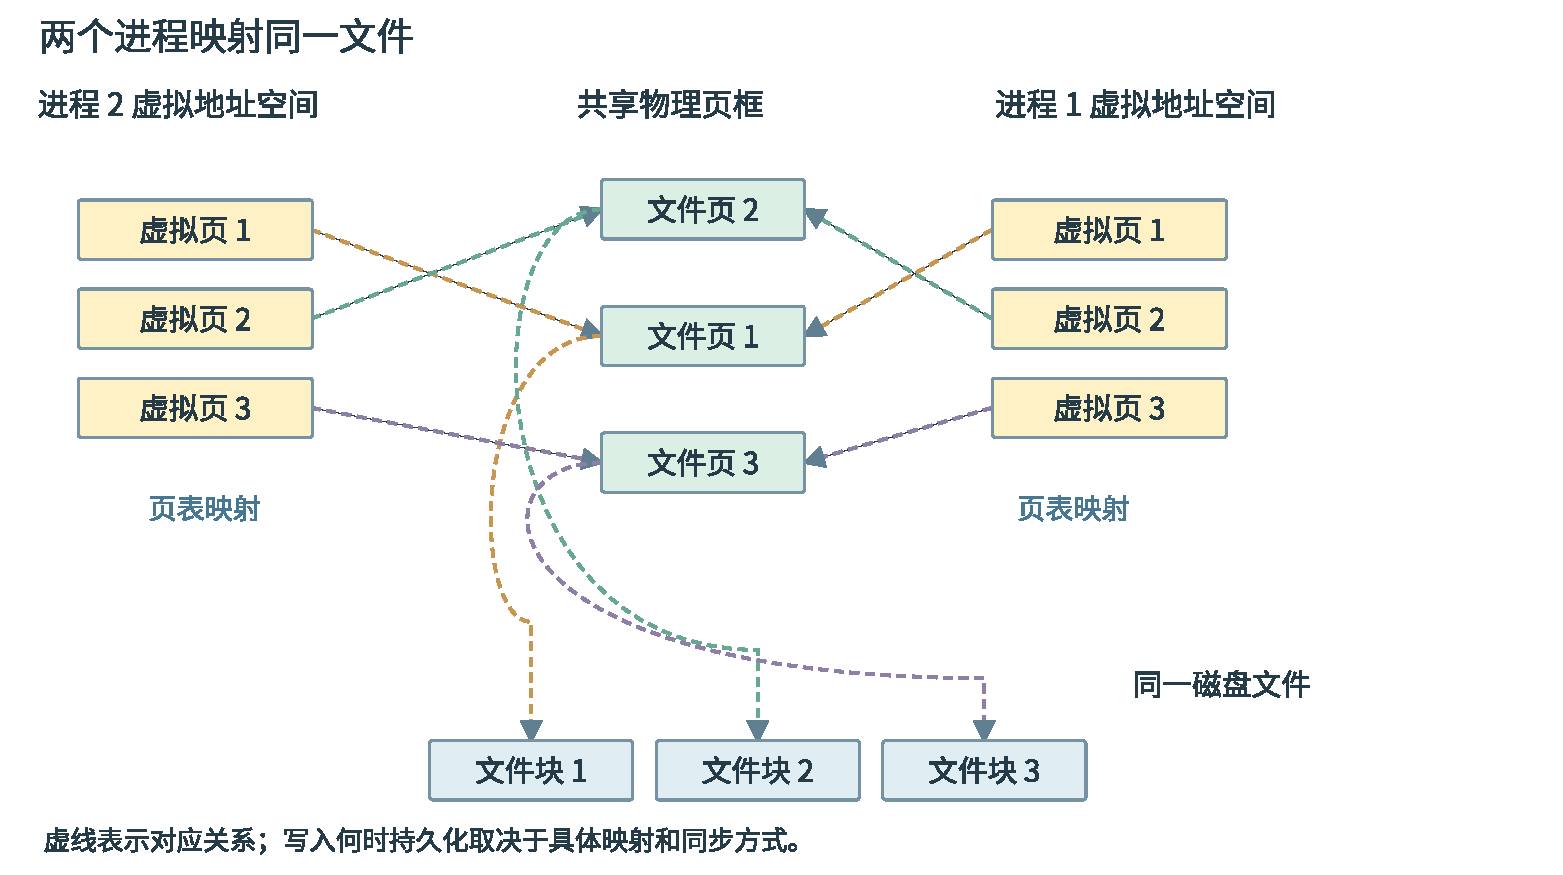
\includegraphics[width=\linewidth,height=125mm,keepaspectratio]{figures/OS03_mmap_shared.pdf}
\captionof{figure}{两个进程的文件页映射到同一组物理页框并对应同一文件块}\label{os03-mmap-shared}
\end{minipage}\par\medskip

\end{wideblock}

映射以后仍受地址范围和权限约束，映射建立、页面驻留、写回持久化是不同事件。题目若问磁盘 I/O 次数，要检查页面是否已缓存、是否发生缺页、脏页是否回写，不能仅按源代码中的读写次数计算。

\Needspace{22\baselineskip}

\section{工作集、抖动与平均访问时间}\label{OS03-5-11}

\textbf{工作集}是在给定窗口内实际访问过的不同页面的集合。若窗口按最近 \(\Delta\) 次引用定义，就从当前位置向前数 \(\Delta\) 次引用，再去重；不能先数 \(\Delta\) 个不同页。驻留集描述当前物理状态，工作集描述近期访问需求，工作集不必总是驻留集的子集：刚被引用、尚未调入的页就可能在工作集中而不在驻留集中。

\textbf{窗口为4的原例。} 页面引用串为 24、15、18、23、24、17、18、24、18、17、17、15。访问完前4项时，窗口含 \(24,15,18,23\)，工作集为 \(\{24,15,18,23\}\)；访问完第10项时，最近4次引用为第7至10项 \(18,24,18,17\)，去重得到 \(\{18,24,17\}\)，工作集大小为3。窗口长度是4，工作集大小可以小于4，因为同一页面可在窗口内重复出现。

\begin{wideblock}

\par\medskip\noindent\begin{minipage}{\linewidth}
\centering
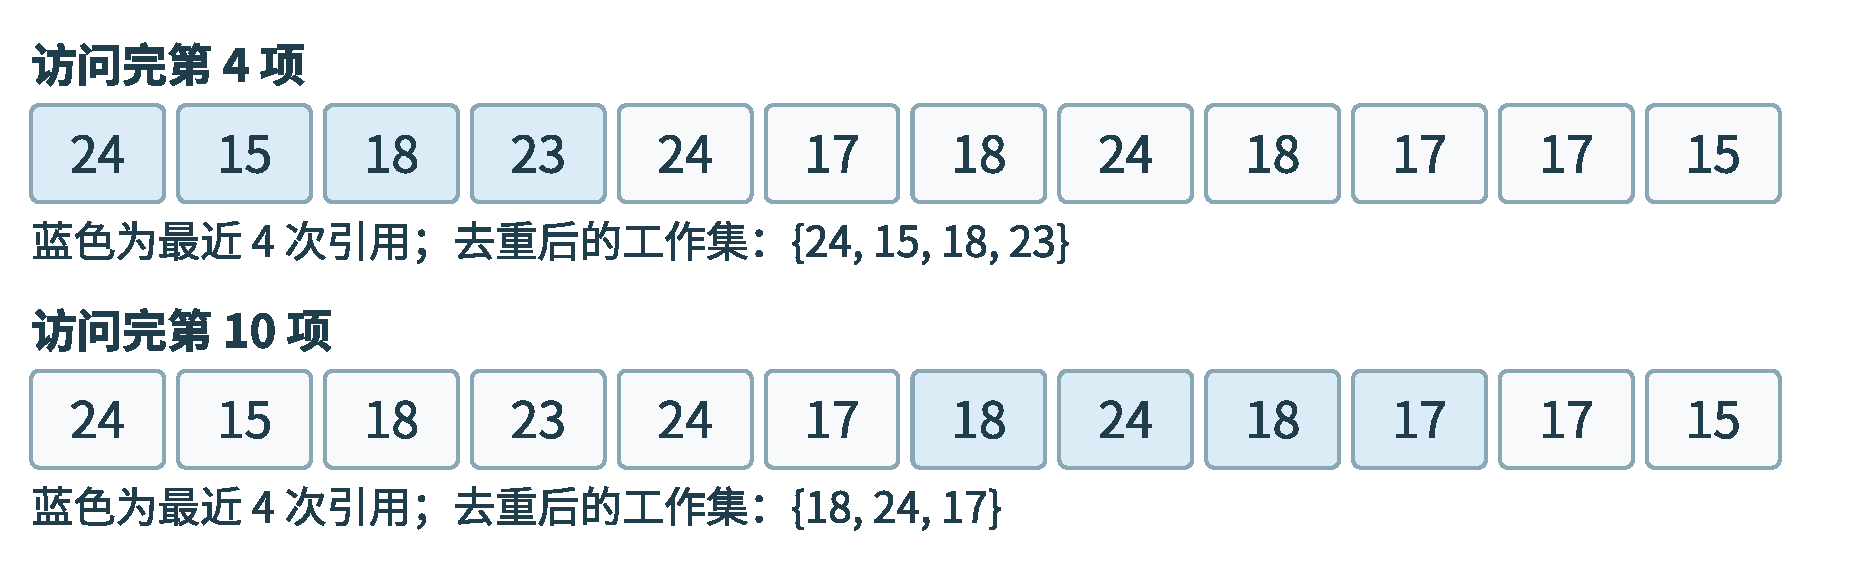
\includegraphics[width=\linewidth,height=125mm,keepaspectratio]{figures/OS03_working_set_course.pdf}
\captionof{figure}{窗口大小为4时，两个时刻的工作集}\label{os03-working-set-course}
\end{minipage}\par\medskip

\end{wideblock}

\subsection{例 3-7　窗口内有重复，集合只记一次}\label{OS03-ex5-7}

\begin{example}[配套例题]

【配套例题】 某进程访问页面的序列如下，t 位于所示竖线处，尚未访问竖线右侧的 0。

\[\ldots,1,3,4,5,6,0,3,2,3,2\;\big|_{t}\;0,4,0,3,2,9,2,1,\ldots\]

工作集窗口大小为 6，则 t 时刻工作集为（　）。

A. \{6,0,3,2\}　　B. \{2,3,0,4\}\\
C. \{0,4,3,2,9\}　　D. \{4,5,6,0,3,2\}

\end{example}

\textbf{解析。} 向前取最近六次引用 6、0、3、2、3、2，去重为 \{6,0,3,2\}，答案为 \textbf{A}。集合无需保留重复次数，也不能从 t 向未来取引用；把窗口理解成``六个不同页面''会错误扩大范围。

\textbf{抖动}指页面频繁换出又很快需要换入，大量时间花在换页，实际计算进展很少。若多进程工作集所需总页框超过可用内存，过度增加并发度可能引发抖动。减少活动进程、增加相关进程的可用页框、依据工作集或缺页率调节分配，才能缓解驻留页框不足；仅扩充磁盘交换区容量或提高某进程优先级，不会自动提供它需要的页框。

\subsection{数组访问怎样变成页引用串}\label{OS03-auto-4}

〖3.2-012〗 页框为 512 B，数组 \texttt{int a[\allowbreak{}128]\allowbreak{}[\allowbreak{}128]\allowbreak{}} 按行优先存放，代码已经驻留，数据只有 1 个页框。下列代码执行会产生多少次缺页？

\par\medskip\noindent\begin{minipage}{\linewidth}
\begin{codeblock}[language=C]
for (int i = 0; i < 128; i++)
    for (int j = 0; j < 128; j++)
        a[j][i] = 0;
\end{codeblock}
\end{minipage}\par\medskip

A. 1　　B. 2\\
C. 128　　D. 16384

\textbf{解析。} 本题采用 4 B 整数，数组按页对齐，数据初始未装入；一行正好 \(128\times4=512\) B，占一页。内层循环 j 增加，访问的是不同的行，即依次跨页；一份数据页框只能留下刚访问的那一行。每次引用都换到另一行，下一列回到第 0 行时，该行那一页也早已被淘汰，因此 \(128\times128=16384\) 次，答案为 \textbf{D}。

这里缺页与置换算法无关，因为只有一个数据页框。若把内层访问改为 \texttt{a[\allowbreak{}i]\allowbreak{}[\allowbreak{}j]\allowbreak{}}，按行连续访问且上述对齐条件不变，每行初次访问缺页一次，总共 128 次。这是\textbf{原创变式}，只改变下标次序，用来检查空间局部性，而非另一道原题。若整数大小、初始驻留或数组页对齐改变，先重建地址和页引用串，再讨论算法，不能只记住 16384 这个数。

\subsection{有效访问时间要列出所有分支}\label{OS03-auto-5}

设不缺页的一次访问平均耗时为 \(T_0\)，缺页率为 \(p\)，一次缺页的完整分支平均耗时为 \(T_f\)，且 \(T_f\) 已包括调页、必要写回、处理程序及重试访问，则

\[E[T]=(1-p)T_0+pT_f.\]

若题目把缺页服务时间 \(D\) 定义成正常访存以外的附加开销，则可写 \(E[T]=T_0+pD\)，两种写法只是费用定义不同。也不能把 TLB 命中率与缺页率相加，当作一个统一的命中率；应按条件概率和完整路径分支。

\textbf{原创计算检查。} 若 \(T_0=100\) ns，缺页完整分支为 10 ms，希望平均访问不超过 200 ns，则

\[p\le\frac{200-100}{10^7-100}\approx10^{-5}.\]

毫秒先换成纳秒，才可与 100 相减。这个数量级说明为什么低缺页率仍可能显著影响时间，不是对任何实机性能的统计结论。

\subsection{例 3-8　一次缺页要把``失败、调页、重试''全部计时}\label{OS03-ex5-8}

\begin{example}[配套例题]

【配套例题】 请求分页管理系统中，假设某进程的页表内容如下表所示。

\begin{wideblock}

\par\medskip\noindent\begin{minipage}{\linewidth}\fontsize{9.3}{12}\selectfont\begin{tabularx}{\linewidth}{@{}YYY@{}}
\toprule\noalign{}
页号 & 页框号 & 有效位（存在位） \\
\midrule\noalign{}


0 & 101H & 1 \\
1 & --- & 0 \\
2 & 254H & 1 \\
\bottomrule\end{tabularx}
\end{minipage}\par\medskip

\end{wideblock}

页面大小为 4 KB，一次内存的访问时间为 100 ns，一次快表（TLB）的访问时间为 10 ns，处理一次缺页的平均时间为 \(10^8\) ns（已含更新 TLB 和页表的时间）。进程的驻留集大小固定为 2，采用最近最少使用置换算法（LRU）和局部淘汰策略。假设：{\SNsymbolfont ①}TLB 初始为空；{\SNsymbolfont ②}地址转换时先访问 TLB，若 TLB 未命中，再访问页表（忽略访问页表之后的 TLB 更新时间）；{\SNsymbolfont ③}有效位为 0 表示页面不在内存中，产生缺页中断，缺页中断处理后，返回到产生缺页中断的指令处重新执行。设有虚地址访问序列 2362H、1565H、25A5H，请问：

（1）依次访问上述三个虚地址，各需多少时间？给出计算过程。

（2）基于上述访问序列，虚地址 1565H 的物理地址是多少？请说明理由。

\end{example}

\textbf{解析。} 4 KB=\(1000_H\) B，低 12 位是页内偏移。三个地址分别访问页 2、页 1、页 2，偏移依次为 362H、565H、5A5H。先连续跟踪这三个访问，不能把每个地址都当作从``TLB 为空''开始。

\begin{wideblock}

\par\medskip\noindent\begin{minipage}{\linewidth}\fontsize{9.3}{12}\selectfont\begin{tabularx}{\linewidth}{@{}YYY@{}}
\toprule\noalign{}
\begin{minipage}[b]{\linewidth}\raggedright
本次访问
\end{minipage} & \begin{minipage}[b]{\linewidth}\raggedright
转换与驻留状态
\end{minipage} & \begin{minipage}[b]{\linewidth}\raggedright
耗时
\end{minipage} \\
\midrule\noalign{}


2362H & TLB 未命中；页 2 驻留，读页表后读目标内存；将页 2 的转换留在 TLB & \(10+100+100=210\) ns \\
1565H & TLB 未命中；页 1 不驻留；处理缺页，更新页表和 TLB；重试时命中 TLB，再读目标内存 & \(10+100+10^8+10+100=100000220\) ns \\
25A5H & 页 2 仍驻留，其转换仍在 TLB，直接命中后读目标内存 & \(10+100=110\) ns \\
\bottomrule\end{tabularx}
\end{minipage}\par\medskip

\end{wideblock}

第二次访问时两个页框已占满，需在本进程的页 0、页 2 中局部淘汰。页 2 刚被第一次访问使用，因此 LRU 选择页 0。将页 1 装入页框 101H，页 0 的存在位清零，并使其旧 TLB 转换失效；页 2 的映射不变。于是

\[PA(1565_H)=101_H\times1000_H+565_H=101565_H.\]

题目把页表、TLB 更新包含在 \(10^8\) ns 中，却明确要求返回原指令重试。因此更新成本不重复加，重试的 10+100 ns 仍须加。第三次访问能命中，也依赖连续执行所得的状态；TLB 未命中、缺页、页面置换是三个不同事件。

\subsection{例 3-9　数组偏移怎样逐级找到页表项}\label{OS03-ex5-9}

\begin{example}[配套例题]

【配套例题】 某 32 位系统采用基于二级页表的请求分页存储管理方式，按字节编址，页目录项和页表项长度均为 4 字节，虚拟地址结构如下所示。

\begin{wideblock}

\par\medskip\noindent\begin{minipage}{\linewidth}\fontsize{9.3}{12}\selectfont\begin{tabularx}{\linewidth}{@{}YYY@{}}
\toprule\noalign{}
页目录号（10 位） & 页号（10 位） & 页内偏移量（12 位） \\
\midrule\noalign{}


\bottomrule\end{tabularx}
\end{minipage}\par\medskip

\end{wideblock}

某 C 程序中数组 \texttt{a[\allowbreak{}1024]\allowbreak{}[\allowbreak{}1024]\allowbreak{}} 的起始虚拟地址为 1080 0000H，数组元素占 4 字节，该程序运行时，其进程的页目录起始物理地址为 0020 1000H。请回答下列问题。

（1）数组元素 \texttt{a[\allowbreak{}1]\allowbreak{}[\allowbreak{}2]\allowbreak{}} 的虚拟地址是什么？对应的页目录号和页号分别是什么？对应的页目录项的物理地址是什么？若该目录项中存放的页框号为 00301H，则 \texttt{a[\allowbreak{}1]\allowbreak{}[\allowbreak{}2]\allowbreak{}} 所在页对应的页表项的物理地址是什么？

（2）数组 a 在虚拟地址空间中所占的区域是否必须连续？在物理地址空间中所占区域是否必须连续？

（3）已知数组 a 按行优先方式存放，若对数组 a 分别按行遍历和按列遍历，则哪种遍历方式的局部性更好？

\end{example}

\textbf{解析。} （1）C 的下标从 0 开始，按行优先存放。到 \texttt{a[\allowbreak{}1]\allowbreak{}[\allowbreak{}2]\allowbreak{}} 的字节偏移为 \((1\times1024+2)\times4=4104=1008_H\)，故其虚拟地址为

\[1080\,0000_H+1008_H=1080\,1008_H.\]

然后按位宽拆分，并把``表项地址''和``表项中保存的页框号''分开计算。

\begin{wideblock}

\par\medskip\noindent\begin{minipage}{\linewidth}\fontsize{9.3}{12}\selectfont\begin{tabularx}{\linewidth}{@{}YYY@{}}
\toprule\noalign{}
所求对象 & 计算 & 结果 \\
\midrule\noalign{}


页目录号 & \(VA\gg22\) & 042H \\
页号（下级表索引） & \((VA\gg12)\mathbin{\&}3FF_H\) & 001H \\
页内偏移 & \(VA\mathbin{\&}FFF_H\) & 008H \\
页目录项物理地址 & \(0020\,1000_H+042_H\times4\) & 0020 1108H \\
下级页表起始物理地址 & \(00301_H\times1000_H\) & 0030 1000H \\
页表项物理地址 & \(0030\,1000_H+001_H\times4\) & 0030 1004H \\
\bottomrule\end{tabularx}
\end{minipage}\par\medskip

\end{wideblock}

题目没有给出这个页表项中的最终页框号，不能把 0030 1004H 当作 \texttt{a[\allowbreak{}1]\allowbreak{}[\allowbreak{}2]\allowbreak{}} 的物理地址；它是下一步需要读取的映射项的位置。

（2）该 C 数组的元素按规定连续排列，所以所占虚拟区域必须连续；相邻虚拟页可映射到离散的页框，物理区域不必连续。页内连续与跨页离散可以同时成立。

（3）每行 \(1024\times4=4096\) B，恰为一页，起始地址也按页对齐。按行遍历在同一页中连续取元素，空间局部性更好；按列遍历的相邻元素相差 4096 B，会逐行跨页。但原题没有给驻留集大小、替换规则和初始状态，不能进一步声称按列必然每次缺页。地址跨度决定访问模式，缺页次数还取决于驻留状态。

\section{分支自测：先写地址字段和状态，再计算}\label{OS03-5-review}

以下为原创回顾设问。

\begin{enumerate}
\def\labelenumi{\arabic{enumi}.}
\tightlist
\item
  32 位虚拟地址、4 KB 页、4 B 页表项，单级页表若覆盖全部空间，需要多少表项和多少字节？
\item
  TLB 未命中而页表存在位为 1，是否一定访问磁盘？存在位为 1、写权限为 0，写访问应怎样处理？
\item
  某页修改位为 0，是否表示程序没有读过该页？
\item
  例 3-5中为何 9 次缺页只有 5 次置换？
\item
  工作集窗口增加，集合大小是否每次恰好增加 1？
\end{enumerate}

\subsection{自测答案}\label{OS03-auto-6}

\begin{enumerate}
\def\labelenumi{\arabic{enumi}.}
\tightlist
\item
  页号 20 位，共 \(2^{20}\) 项，占 \(2^{22}\) B，即 4 MB；这与物理页框总数不是同一个计算。
\item
  未命中可通过主存页表取得映射，不必读盘。写权限不足应触发保护异常，不能当作普通缺页调入后允许写。
\item
  否。读访问可以使访问位置 1，却不使修改位置 1。
\item
  最初四次使用空闲页框，尚未淘汰任何页；之后满框缺页才置换。
\item
  不会。新纳入的一次引用可能已在集合中，窗口内重复引用只算同一个页。
\end{enumerate}

\section{主动回忆自测}\label{OS03-recall}

以下为自拟回忆题，先画地址字段或状态，再写结论。

\begin{recallcard}[从合法地址追踪到完整费用]

\begin{enumerate}
\def\labelenumi{\arabic{enumi}.}
\tightlist
\item
  虚拟地址宽32位，页4KiB，页表项4B，覆盖全部虚拟空间的单级页表有多少项、占多少空间？
\item
  两个各6MiB的不相邻空洞，能否满足连续8MiB请求？分页消除了哪类碎片，又留下哪类？
\item
  页大小1KiB，虚拟地址0A6FH，页2映射到页框BH，物理地址是多少？
\item
  二级页表TLB命中率75\%，忽略TLB耗时且无缺页，每次查询均串行，平均需几次主存访问？
\item
  段已驻留且可写，段长300，偏移400，能否访问基址加400？
\item
  两页框访问A、B、A、C，LRU与FIFO分别淘汰谁？
\item
  缺页9次，其中4次使用初始空页框，置换多少次？何时还要计算回写？
\item
  解释工作集、驻留集、内存映射建立、脏页写回四个概念为什么不能混用。
\end{enumerate}

\end{recallcard}

\subsection{核对答案与计算}\label{OS03-recall-answers}

\begin{enumerate}
\def\labelenumi{\arabic{enumi}.}
\tightlist
\item
  页内偏移12位，虚拟页号20位，共\(2^{20}\)项，占\(2^{22}\)B，即4MiB；物理地址宽度影响表项中页框号，而非虚拟页数。
\item
  不能，连续洞不够大。分页消除对整个进程连续分配产生的外部碎片，最后一页仍可能有内部碎片，页表也有开销。
\item
  \(A6F_H=2\times400_H+26F_H\)，偏移保持\(26F_H\)，结果\(B\times400_H+26F_H=2E6F_H\)。
\item
  命中1次读数据，未命中2次查表加1次读数据；\(0.75\times1+0.25\times3=1.5\)次。若查询并行或有缺页须重新列路径。
\item
  不能。\(400\ge300\)越界，驻留与可写均不撤销段长检查。
\item
  命中A使它在LRU中最近，故淘汰B；FIFO仍按装入先后淘汰A。
\item
  置换5次；被淘汰页若脏且需保留内容，应另计写回，服务时间已包含时不重复加。
\item
  工作集是近期需求集合，驻留集是当前物理状态；建立文件映射规定地址与后备关系，不代表所有页驻留；脏页写回实现相应持久化，发生时刻另由机制决定。
\end{enumerate}
